
%%%%%%%%%%%%%%%%%%%%%%%%%%%%%%%%%%%%%%%%%%%%%%%%%%%%%%%%%%%%%%%%%%%%%
%% This is a (brief) model paper using the achemso class
%% The document class accepts keyval options, which should include
%% the target journal and optionally the manuscript type.
%%%%%%%%%%%%%%%%%%%%%%%%%%%%%%%%%%%%%%%%%%%%%%%%%%%%%%%%%%%%%%%%%%%%%
\documentclass[journal=jacsat,manuscript=article]{achemso}

%%%%%%%%%%%%%%%%%%%%%%%%%%%%%%%%%%%%%%%%%%%%%%%%%%%%%%%%%%%%%%%%%%%%%
%% Place any additional packages needed here.  Only include packages
%% which are essential, to avoid problems later. Do NOT use any
%% packages which require e-TeX (for example etoolbox): the e-TeX
%% extensions are not currently available on the ACS conversion
%% servers.
%%%%%%%%%%%%%%%%%%%%%%%%%%%%%%%%%%%%%%%%%%%%%%%%%%%%%%%%%%%%%%%%%%%%%
\usepackage[version=3]{mhchem} % Formula subscripts using \ce{}
\usepackage{subfig}

%%%%%%%%%%%%%%%%%%%%%%%%%%%%%%%%%%%%%%%%%%%%%%%%%%%%%%%%%%%%%%%%%%%%%
%% If issues arise when submitting your manuscript, you may want to
%% un-comment the next line.  This provides information on the
%% version of every file you have used.
%%%%%%%%%%%%%%%%%%%%%%%%%%%%%%%%%%%%%%%%%%%%%%%%%%%%%%%%%%%%%%%%%%%%%
%%\listfiles

%%%%%%%%%%%%%%%%%%%%%%%%%%%%%%%%%%%%%%%%%%%%%%%%%%%%%%%%%%%%%%%%%%%%%
%% Place any additional macros here.  Please use \newcommand* where
%% possible, and avoid layout-changing macros (which are not used
%% when typesetting).
%%%%%%%%%%%%%%%%%%%%%%%%%%%%%%%%%%%%%%%%%%%%%%%%%%%%%%%%%%%%%%%%%%%%%
\newcommand*\mycommand[1]{\texttt{\emph{#1}}}

%%%%%%%%%%%%%%%%%%%%%%%%%%%%%%%%%%%%%%%%%%%%%%%%%%%%%%%%%%%%%%%%%%%%%
%% Meta-data block
%% ---------------
%% Each author should be given as a separate \author command.
%%
%% Corresponding authors should have an e-mail given after the author
%% name as an \email command. Phone and fax numbers can be given
%% using \phone and \fax, respectively; this information is optional.
%%
%% The affiliation of authors is given after the authors; each
%% \affiliation command applies to all preceding authors not already
%% assigned an affiliation.
%%
%% The affiliation takes an option argument for the short name.  This
%% will typically be something like "University of Somewhere".
%%
%% The \altaffiliation macro should be used for new address, etc.
%% On the other hand, \alsoaffiliation is used on a per author basis
%% when authors are associated with multiple institutions.
%%%%%%%%%%%%%%%%%%%%%%%%%%%%%%%%%%%%%%%%%%%%%%%%%%%%%%%%%%%%%%%%%%%%%
\author{Wangfei Yang}
\affiliation{Systems, Synthetic and Physical Biology Program, Rice University, Houston, TX, USA}
\altaffiliation{Center for Theoretical Biological Physics, Rice University, Houston, TX, USA}

\author{Lorenzo Boninsegna}
\affiliation{Department of Chemistry, Rice University, Houston, TX, USA}
\altaffiliation{Center for Theoretical Biological Physics, Rice University, Houston, TX, USA}

\author{Wenwei Zheng}
\affiliation{College of Integrative Sciences and Arts, Arizona State University, Mesa, AZ, USA}

\author{Cecilia Clementi}
\email{cecilia@rice.edu}
\affiliation{Department of Chemistry, Rice University, Houston, TX, USA}
\altaffiliation{Center for Theoretical Biological Physics, Rice University, Houston, TX, USA}

%%%%%%%%%%%%%%%%%%%%%%%%%%%%%%%%%%%%%%%%%%%%%%%%%%%%%%%%%%%%%%%%%%%%%
%% The document title should be given as usual. Some journals require
%% a running title from the author: this should be supplied as an
%% optional argument to \title.
%%%%%%%%%%%%%%%%%%%%%%%%%%%%%%%%%%%%%%%%%%%%%%%%%%%%%%%%%%%%%%%%%%%%%
\title[An \textsf{achemso} demo]
  {An Investigation on How Dynamics of macromolecules Influence Their Assembly Units with a Data-driven Approach}

%%%%%%%%%%%%%%%%%%%%%%%%%%%%%%%%%%%%%%%%%%%%%%%%%%%%%%%%%%%%%%%%%%%%%
%% Some journals require a list of abbreviations or keywords to be
%% supplied. These should be set up here, and will be printed after
%% the title and author information, if needed.
%%%%%%%%%%%%%%%%%%%%%%%%%%%%%%%%%%%%%%%%%%%%%%%%%%%%%%%%%%%%%%%%%%%%%
%\abbreviations{IR,NMR,UV}
%\keywords{American Chemical Society, \LaTeX}

\begin{document}
%%%%%%%%%%%%%%%%%%%%%%%%%%%%%%%%%%%%%%%%%%%%%%%%%%%%%%%%%%%%%%%%%%%%%
%% The manuscript does not need to include \maketitle, which is
%% executed automatically.  The document should begin with an
%% abstract, if appropriate.  If one is given and should not be, the
%% contents will be gobbled.
%%%%%%%%%%%%%%%%%%%%%%%%%%%%%%%%%%%%%%%%%%%%%%%%%%%%%%%%%%%%%%%%%%%%%
\begin{abstract}
  Biomacromolecules always contain a very large number of degrees of freedom in an atomic resolution. Finding a coarser representation which captures the long-timescale dynamics is significant for investigating the characteristics of the molecule and constructing effective coarse-grained models. Here we investigate how different dynamics of proteins will influence their dynamically assembly units with a recently developed data-driven decomposition algorithm, {\it Structure and State Space Decomposition}. We also propose a modified version of this algorithm to extend its applications on intrinsically disordered proteins. The results from different proteins with similar dynamics show a consistency. Interestingly, the results also show that the dynamical decompositions for specific human-designed proteins and intrinsically disordered proteins significantly differ from the results from other good folders.
\end{abstract}

%%%%%%%%%%%%%%%%%%%%%%%%%%%%%%%%%%%%%%%%%%%%%%%%%%%%%%%%%%%%%%%%%%%%%
%% Start the main part of the manuscript here.
%%%%%%%%%%%%%%%%%%%%%%%%%%%%%%%%%%%%%%%%%%%%%%%%%%%%%%%%%%%%%%%%%%%%%
\section{Introduction}
Thanks to recent developments of our computational power, now we are able to perform molecular dynamics (MD) simulations for biomacromolecules of considerable size on a time-scale of milliseconds, which is the typical timescale for biomolecular processes such as protein folding and ligand binding\cite{MD_simulation}, with an atomic resolution\cite{DE_Shaw_fast-folding,Anton}. However, our computational power is still limited to allowing us to use the same method for larger systems or longer timescales. Fortunately, empirical results and theoretical researches indicate that for most biomacromolecular processes only a little part of the phase space is highly relevant, and the rest consists the fast and local fluctuations\cite{Cecilia_reaction_coordinate_review,Cecilia_low_dimension}. Thus, we can overcome the computational limitation by constructing coarse-grained (CG) models, which conserve the most ``interesting'' portion but wipes off the noise pretty much\cite{AWSEM,MARTINI,Voth_CG_review,CG_methods}. To construct such a model, first we need to identify the subset of the phase space that is highly relevant to the processes we're interested in and the corresponding collective variables can be used as the representation.

Most currently employed CG models reduce the complexity based on the structural modularity of the molecule\cite{CG_model_review}. For example, $C_{\alpha}\&C_{\beta}$ mapping is very popular for CG protein models\cite{structure_based_model,SMOG}. However, a general solution on how to select the optimal collective variables which can reproduce the long timescale dynamics is hardly available, because the dynamical characteristics of the system has a significant influence on the optimal choice of effective degrees of freedom. Recently, a data-driven algorithm called {\it Structure and State Space Decomposition} (S3D) has been developed by Boninsegna {\it et al.} to decompose biomacromolecules into dynamically assembly units based on their all-atom simulation data\cite{Lrenzo_S3D}. This algorithm provides us a method to obtain CG representations case-by-case. Moreover, how dynamics of biomacromolecules influence the choice of effective degrees of freedom can also be investigated by comparing the distributions of assembly units from different systems.

As indicated by its name, S3D performs decompositions in both structure and state space. By decompose the state space, the system's dynamics can be represented as a Markov state model (MSM) composed by few metastable states and the transition rates between them\cite{TICA,TICA_commute_map,TICA_collective_variable,MSM,HMM}. Then in ,the structure space, groups of atoms that preserve their geometric integrity under time evolution are obtained as the dynamically coherent domains for each metastable state by a time-averaged diffusion map approach\cite{diffusion_map_clustering,diffusion_map}. Since we will obtain different coherent domains from different metastable states, the transitions between metastable states can be treated as the splittings and mergings of the coherent domains. Thus, we can easily determine the minimal assembly units as the intersections of the coherent domains from all the metastable states, which always act as a whole\cite{Lrenzo_S3D}. The detailed work flow can be found in the supplementary material.

We here investigate the influence of dynamics of proteins on their assembly units by applying S3D algorithm on a set of 10 fast-folding proteins\cite{DE_Shaw_fast-folding} and 2 intrinsically disordered proteins (IDPs)\cite{ACTR,MYC}. While since we found it is hard to construct a MSM to identify the metastable states for IDPs, we also propose a modified version of S3D to extend the application. The results show that though the minimal assembly units vary in size and position, for good folders, their average size always locates in a specific range. However, if the dynamics of the protein differs in some way, the average size of assembly units will also change correspondingly. For the IDPs, the decomposition results from 2 different proteins are consist, but we find that a set of minimal assembly units which works universally is hard to obtain because of the inexistence of metastable states.

\section{Results and discussion}

\subsection{Fast Folding Proteins}

We first applied this algorithm on a set of 10 fast-folding proteins whose long equilibrium all-atom simulation data are available\cite{DE_Shaw_fast-folding}. The decomposition results are shown in fig-\ref{all_beads}. The detailed data of metastable states and corresponding coherent domains can be found in the supplementary material. The proteins are decomposed into several assembly units, which vary in size and position. Notably, the numbers of assembly units of these proteins are all less than the numbers of their residues. This indicates that through appropriate selection we may be able to capture the long-timescale dynamics of proteins with a smaller number of degrees of freedom than the traditional intuitive methods such as $C_{\alpha}$ or $C_{\alpha}-C_{\beta}$ mapping.

\begin{figure}[htbp]
  \centering
  \subfloat[Chignolin]{
  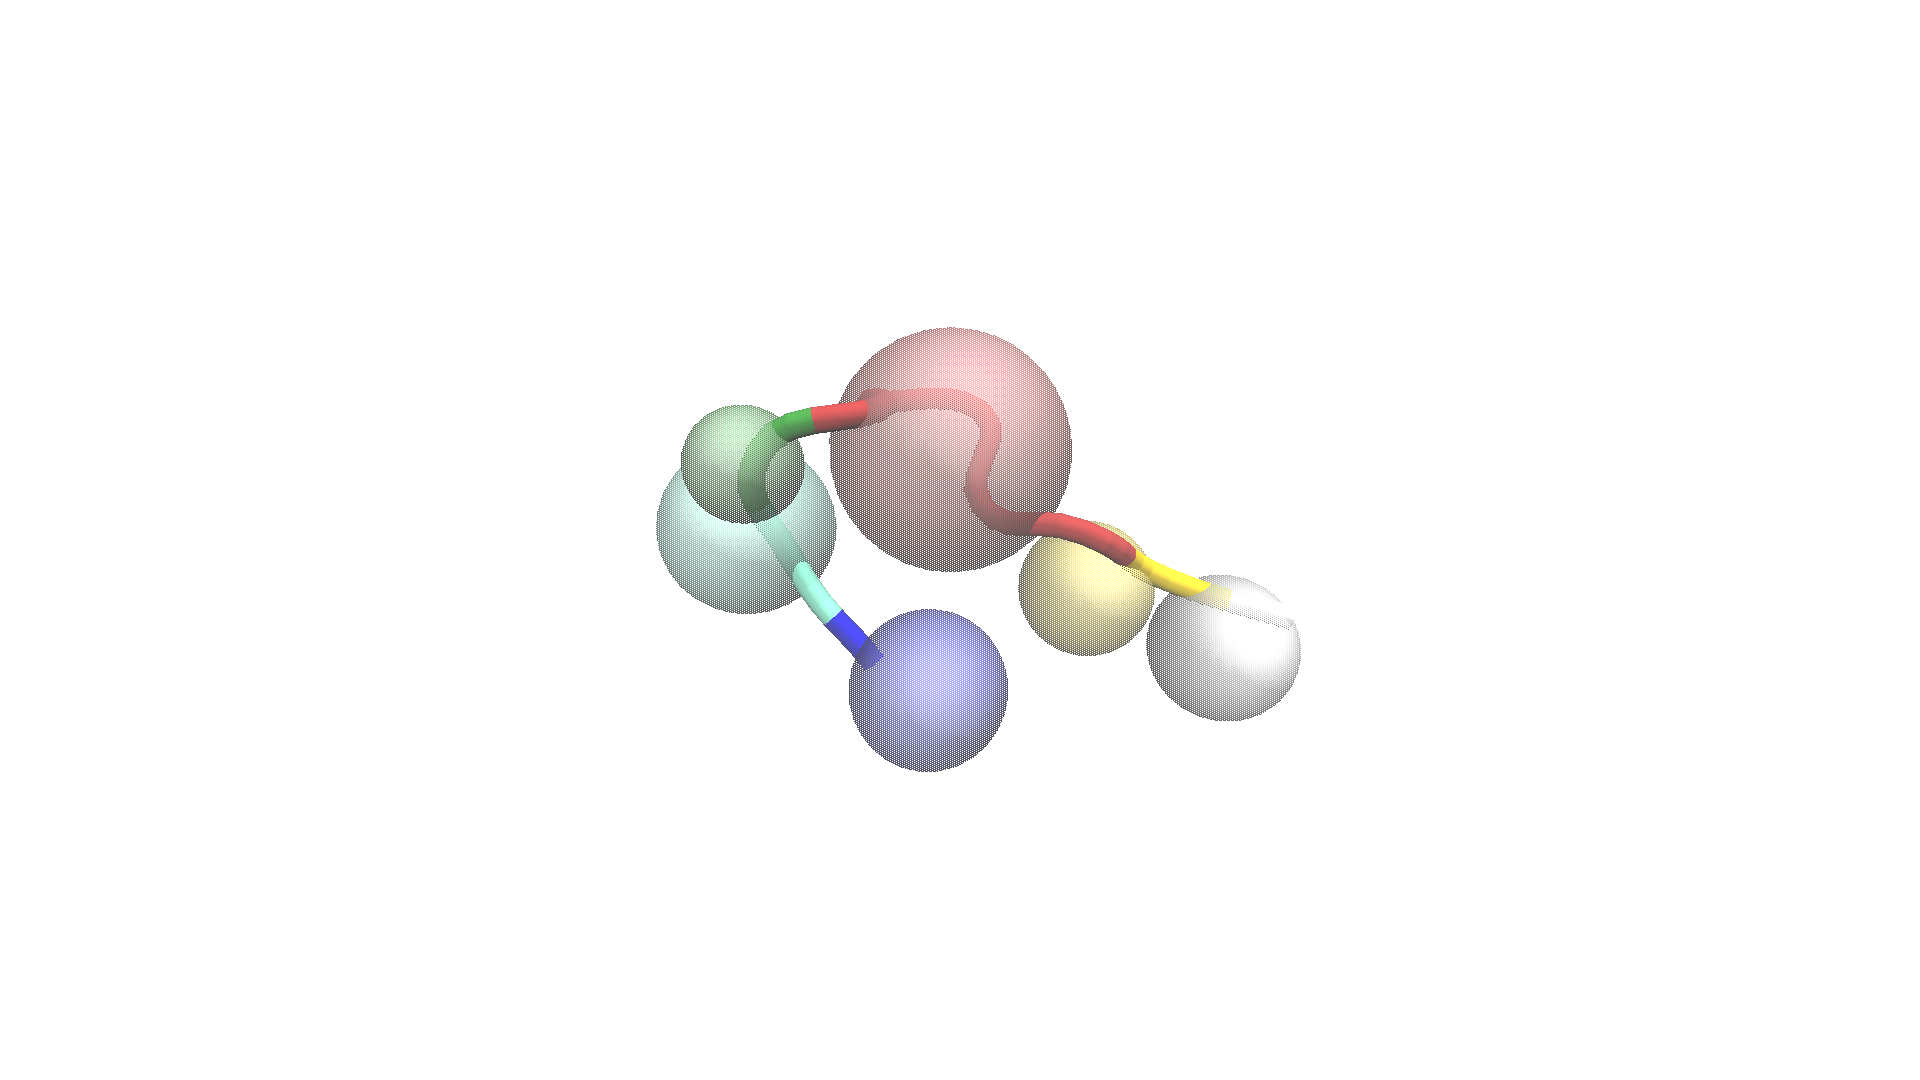
\includegraphics[width=0.25\textwidth, trim={22cm 6cm 22cm 6cm},clip]{CLN025_chignolin_beads.png}}
  \subfloat[Trp-cage]{
  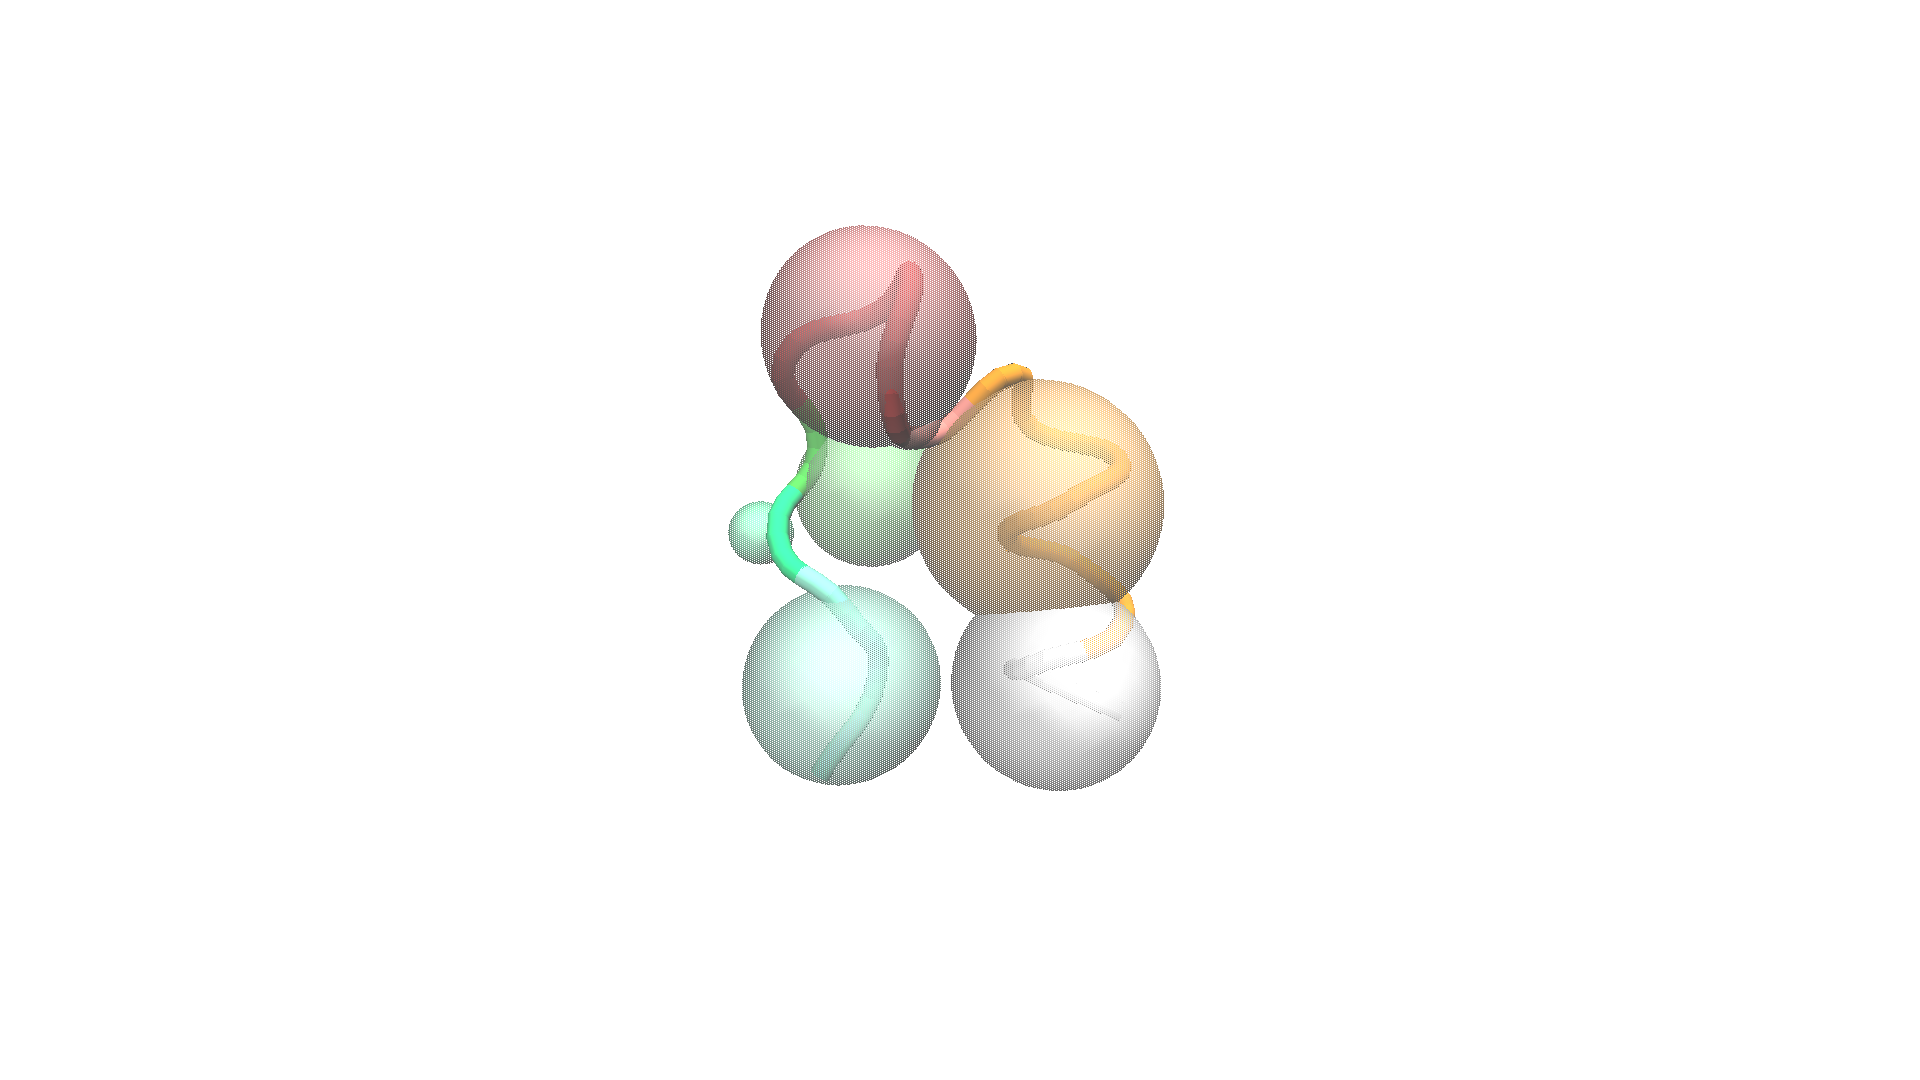
\includegraphics[width=0.25\textwidth, trim={22cm 6cm 22cm 6cm},clip]{2JOF_trp-cage_beads.png}}
  \subfloat[BBA]{
  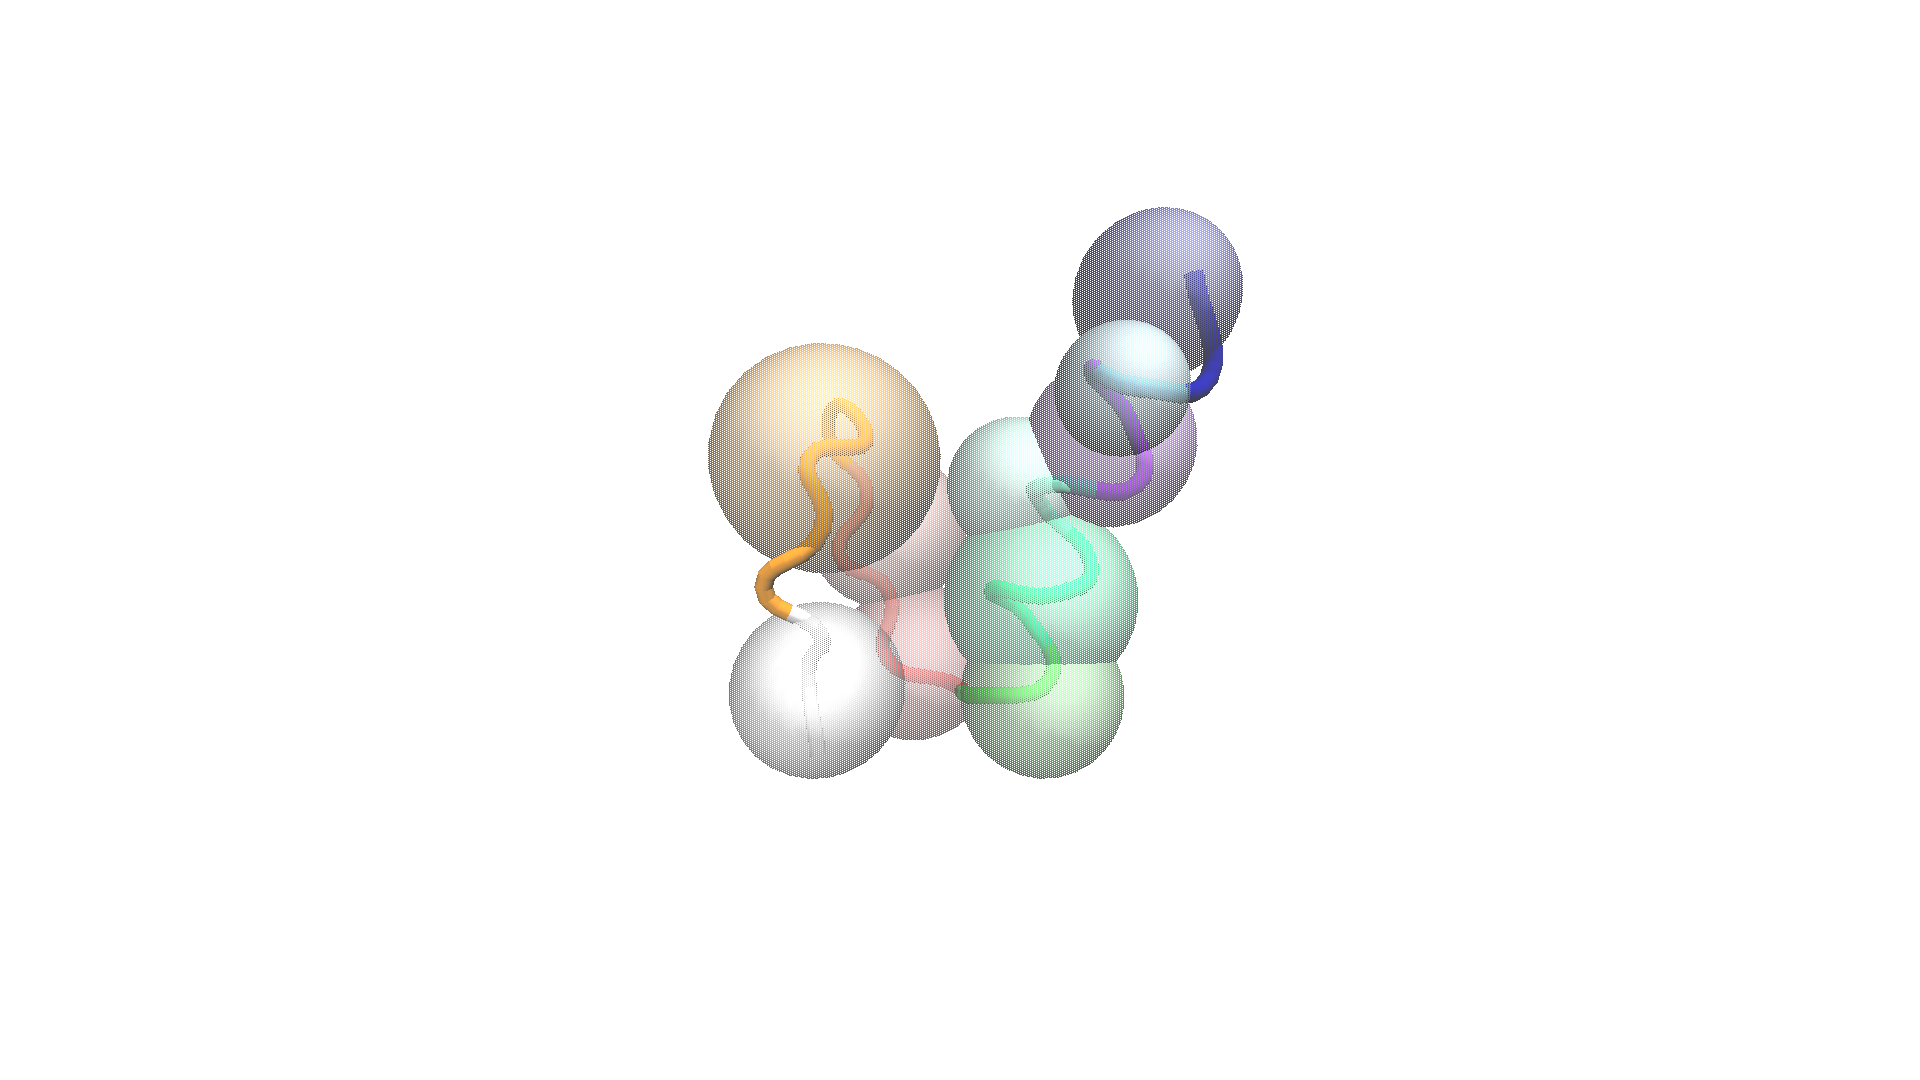
\includegraphics[width=0.25\textwidth, trim={22cm 6cm 22cm 6cm},clip]{1FME_BBA_beads.png}}
  \subfloat[Villin]{
  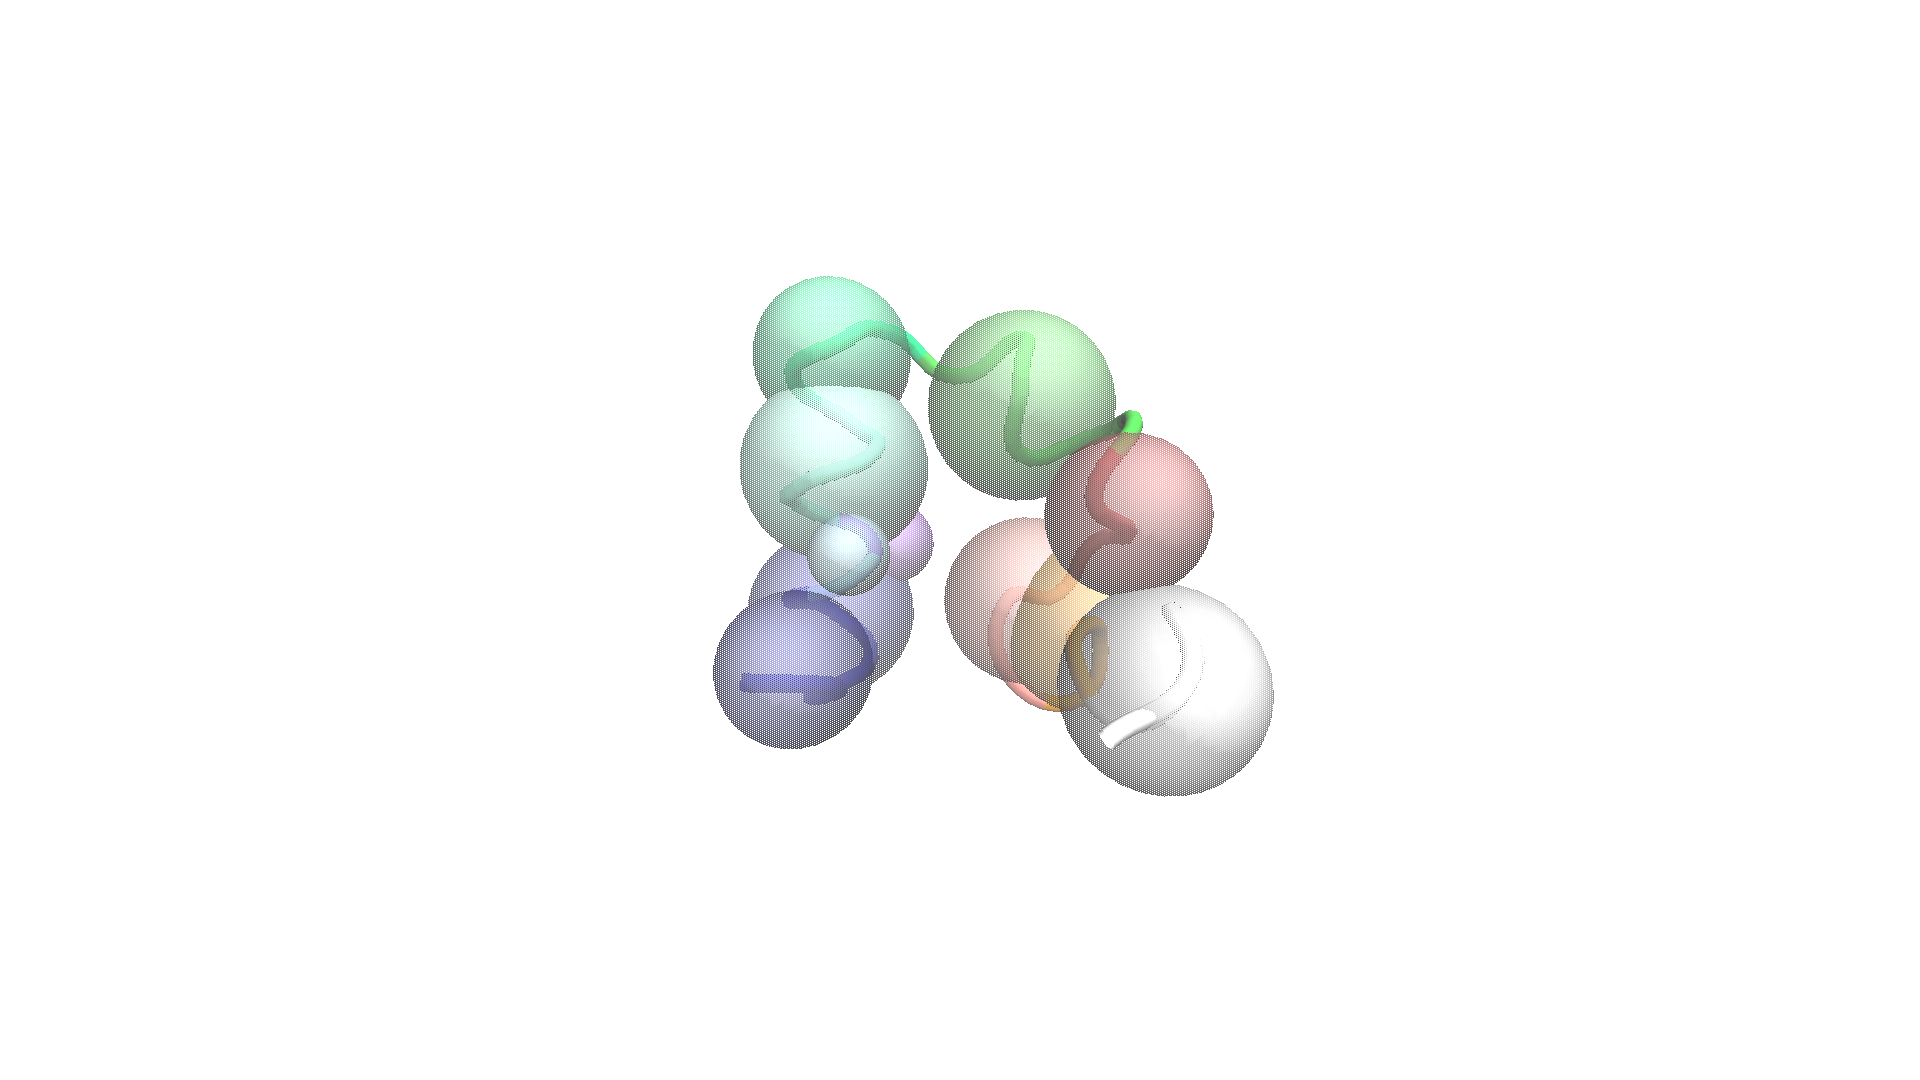
\includegraphics[width=0.25\textwidth, trim={22cm 6cm 22cm 6cm},clip]{2F4K_villin_beads.png}}\\
  \subfloat[BBL]{
  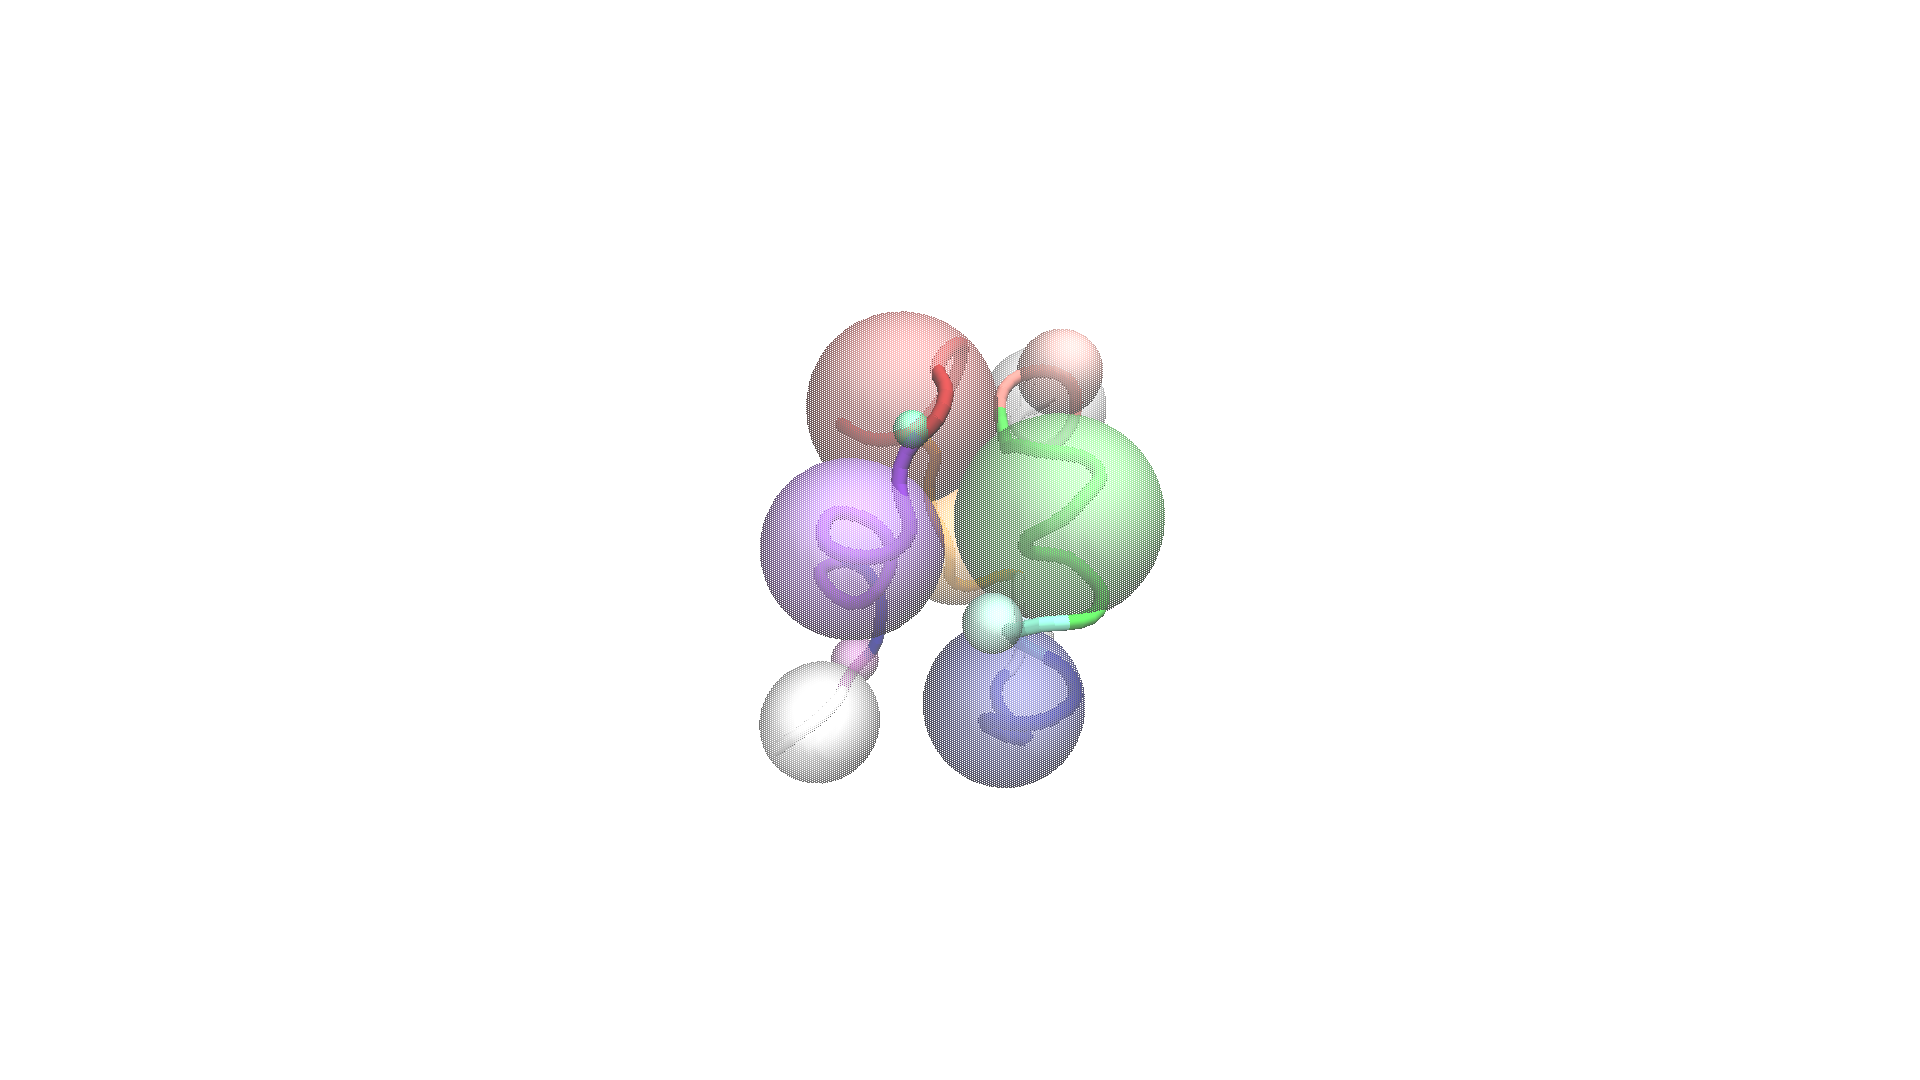
\includegraphics[width=0.25\textwidth, trim={22cm 6cm 22cm 6cm},clip]{2WAV_BBL_beads.png}}
  \subfloat[Protein B]{
  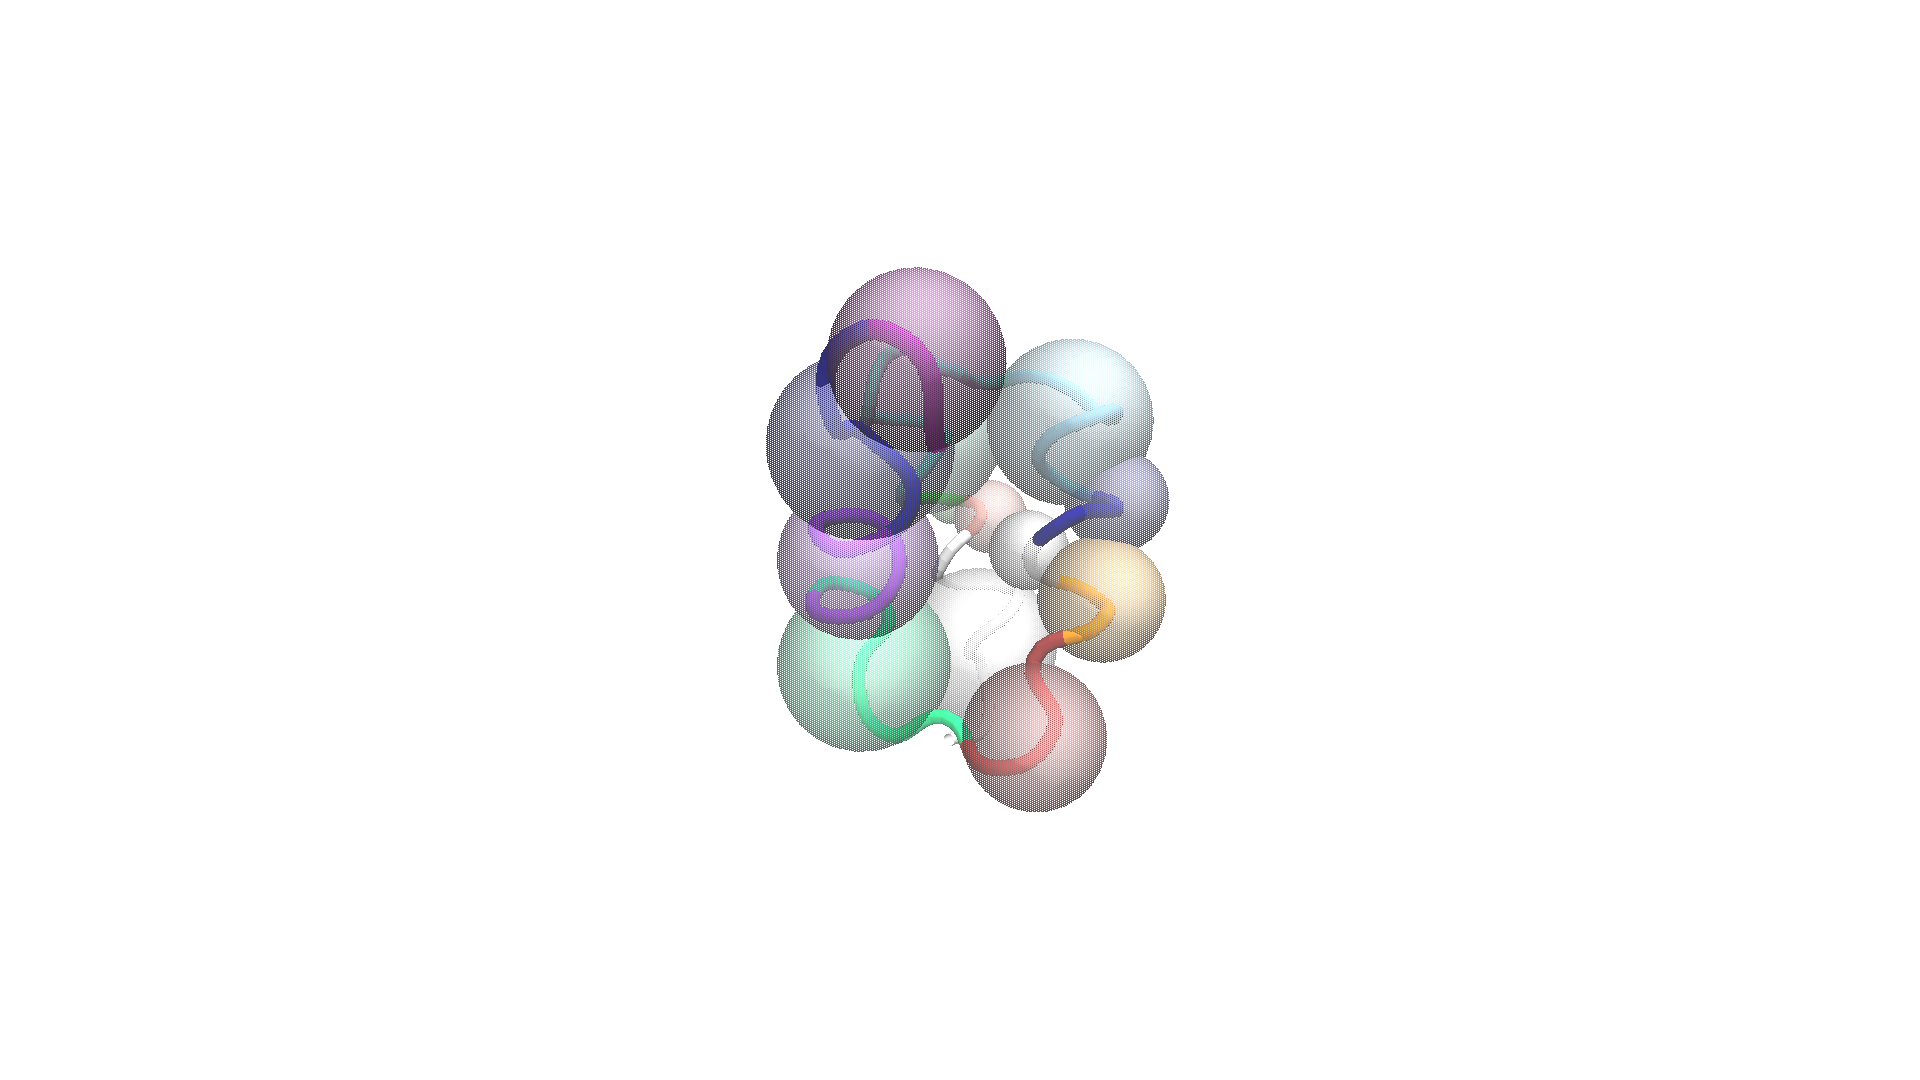
\includegraphics[width=0.25\textwidth, trim={22cm 6cm 22cm 6cm},clip]{PRB_protein_b_beads.png}}
  \subfloat[Homeodomain]{
  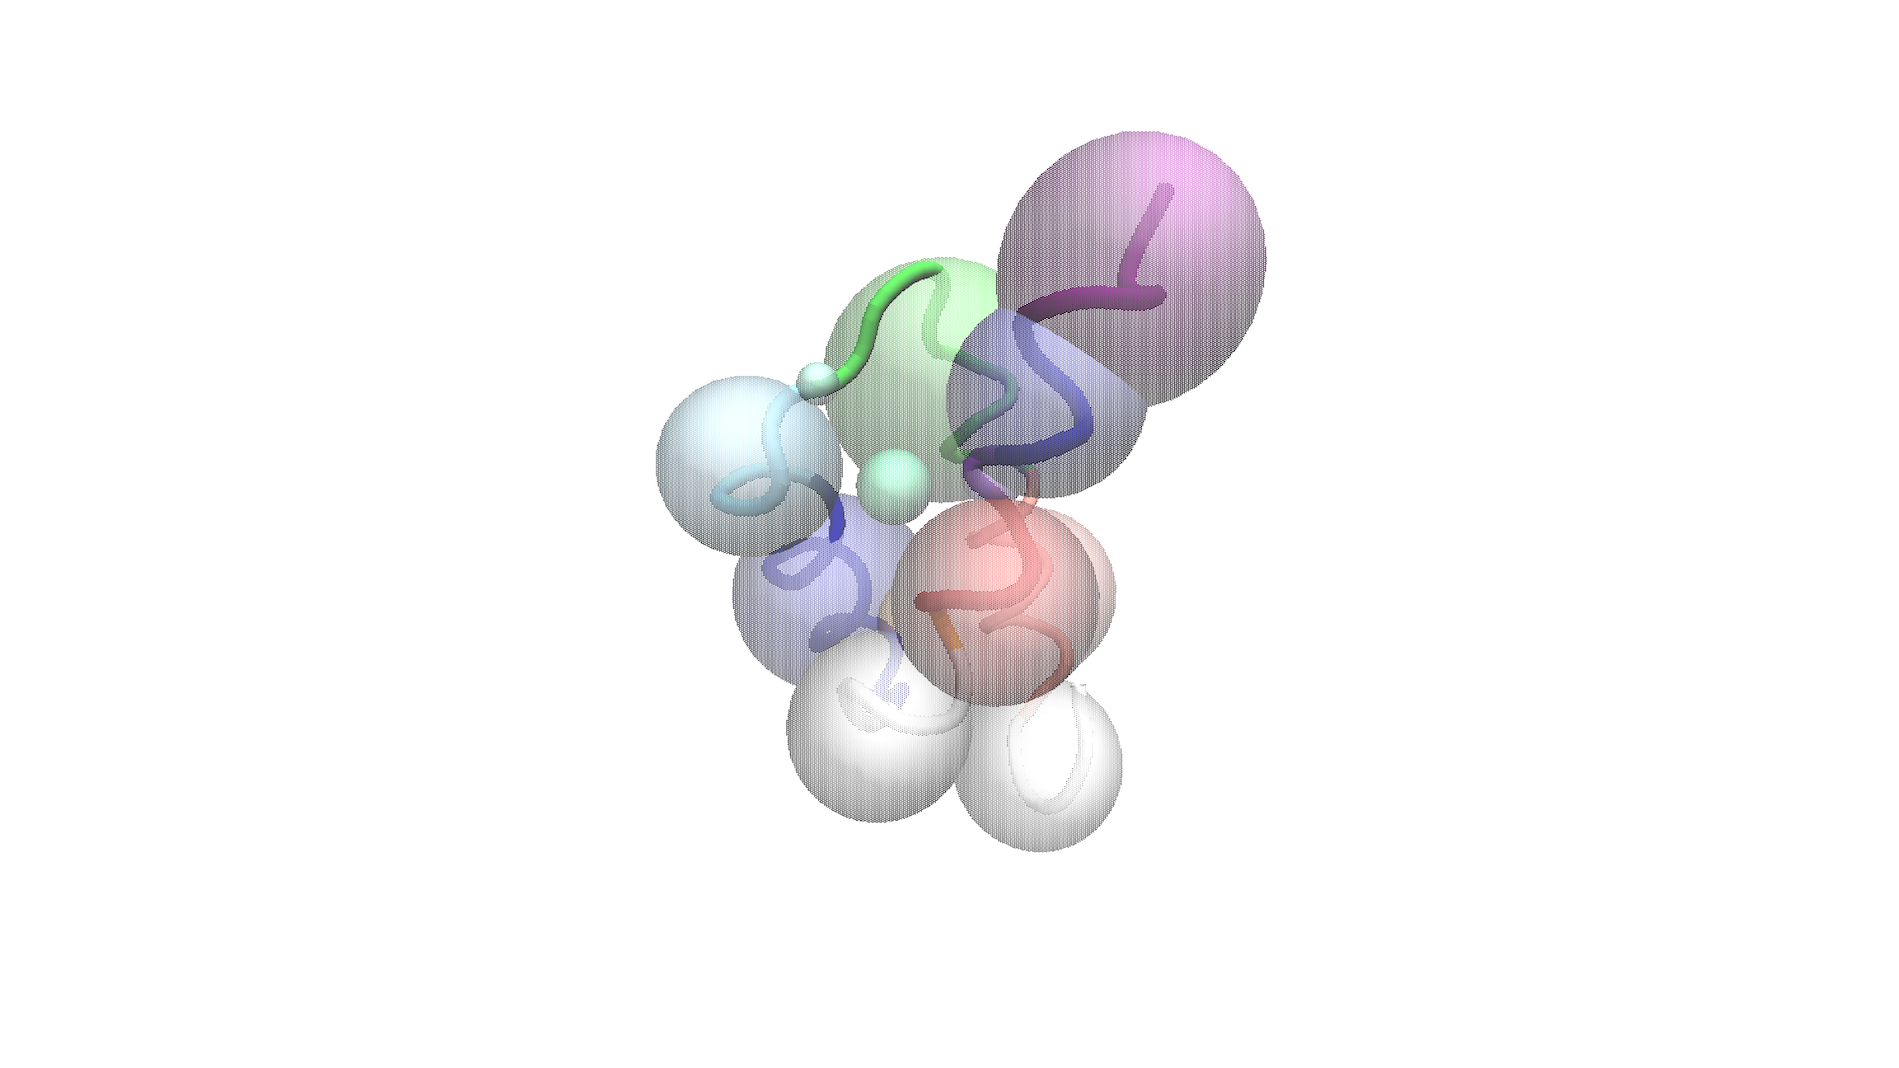
\includegraphics[width=0.25\textwidth, trim={18cm 3cm 18cm 3cm},clip]{UVF_homeodomain_beads.png}}
  \subfloat[Protein G]{
  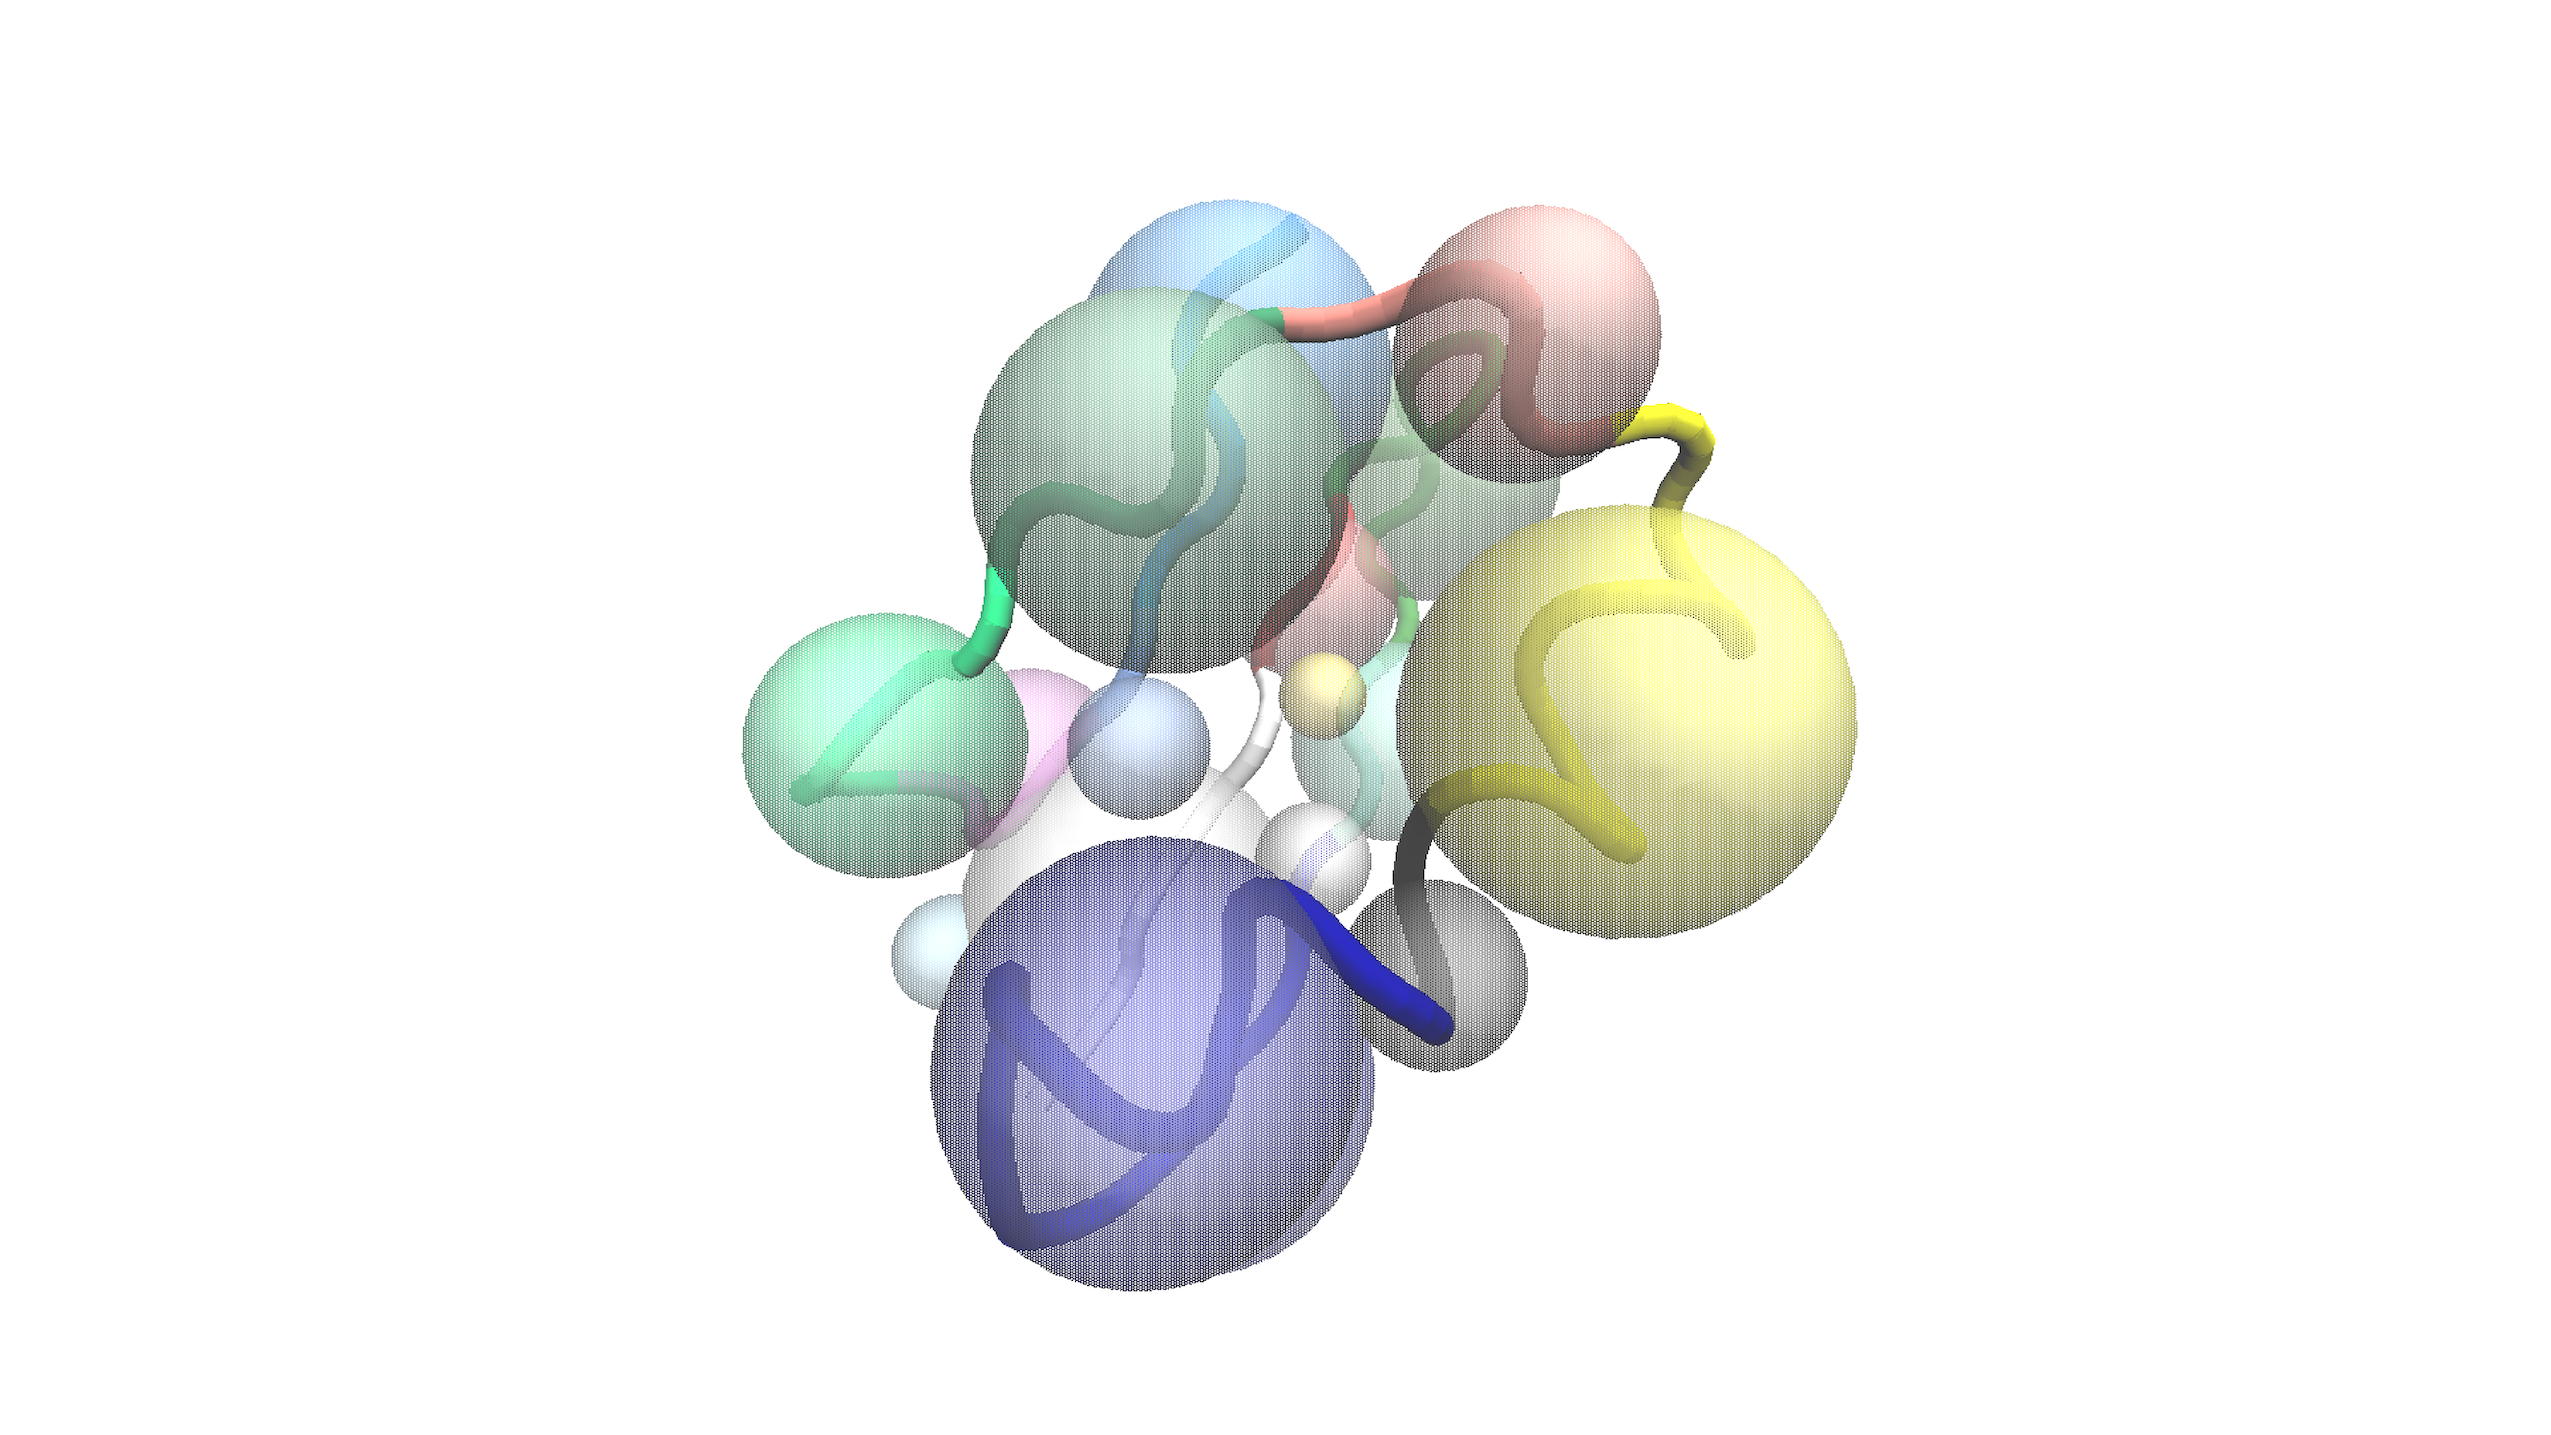
\includegraphics[width=0.25\textwidth, trim={18cm 3cm 18cm 3cm},clip]{NuG2_protein_g_all_beads_new.png}}\\
  \subfloat[$\alpha$3D]{
  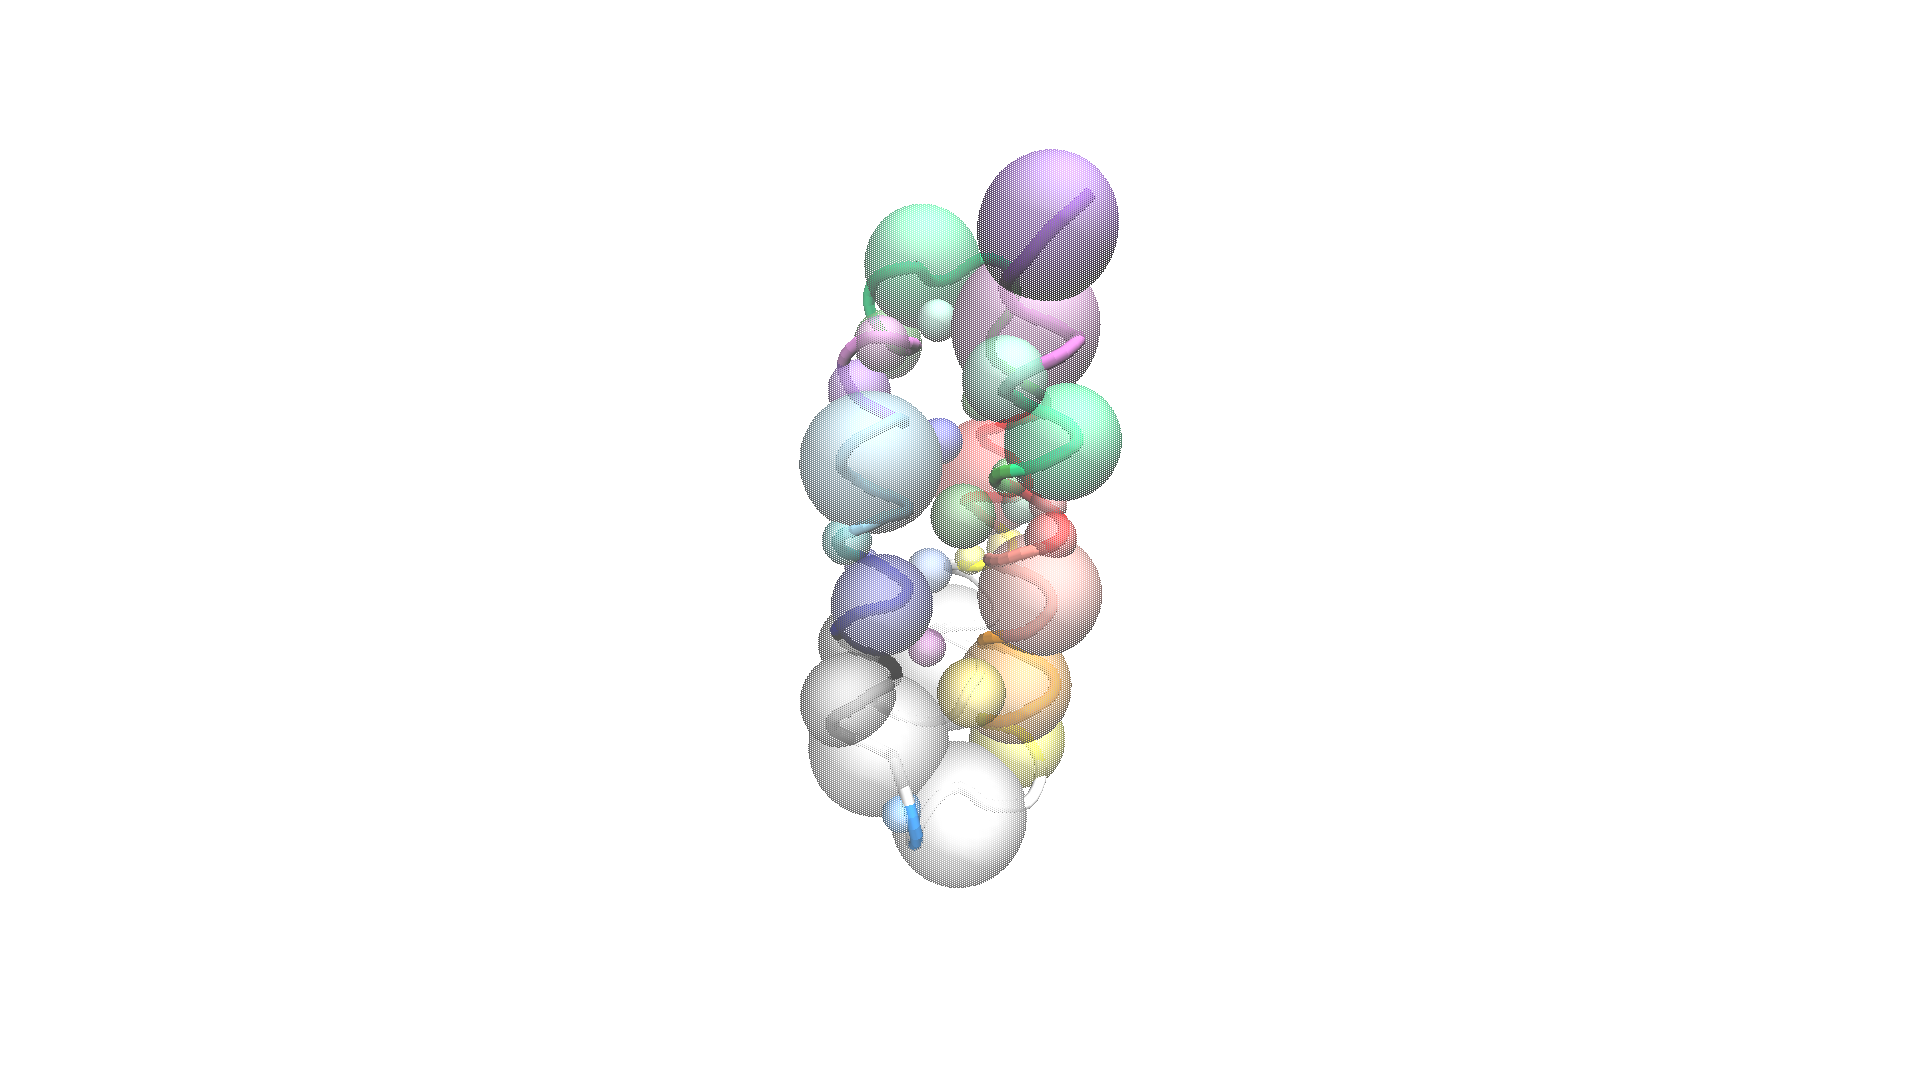
\includegraphics[width=0.25\textwidth, trim={22cm 6cm 22cm 3cm},clip]{A3D_alpha3D_beads.png}}
  \subfloat[$\lambda$-repressor]{
  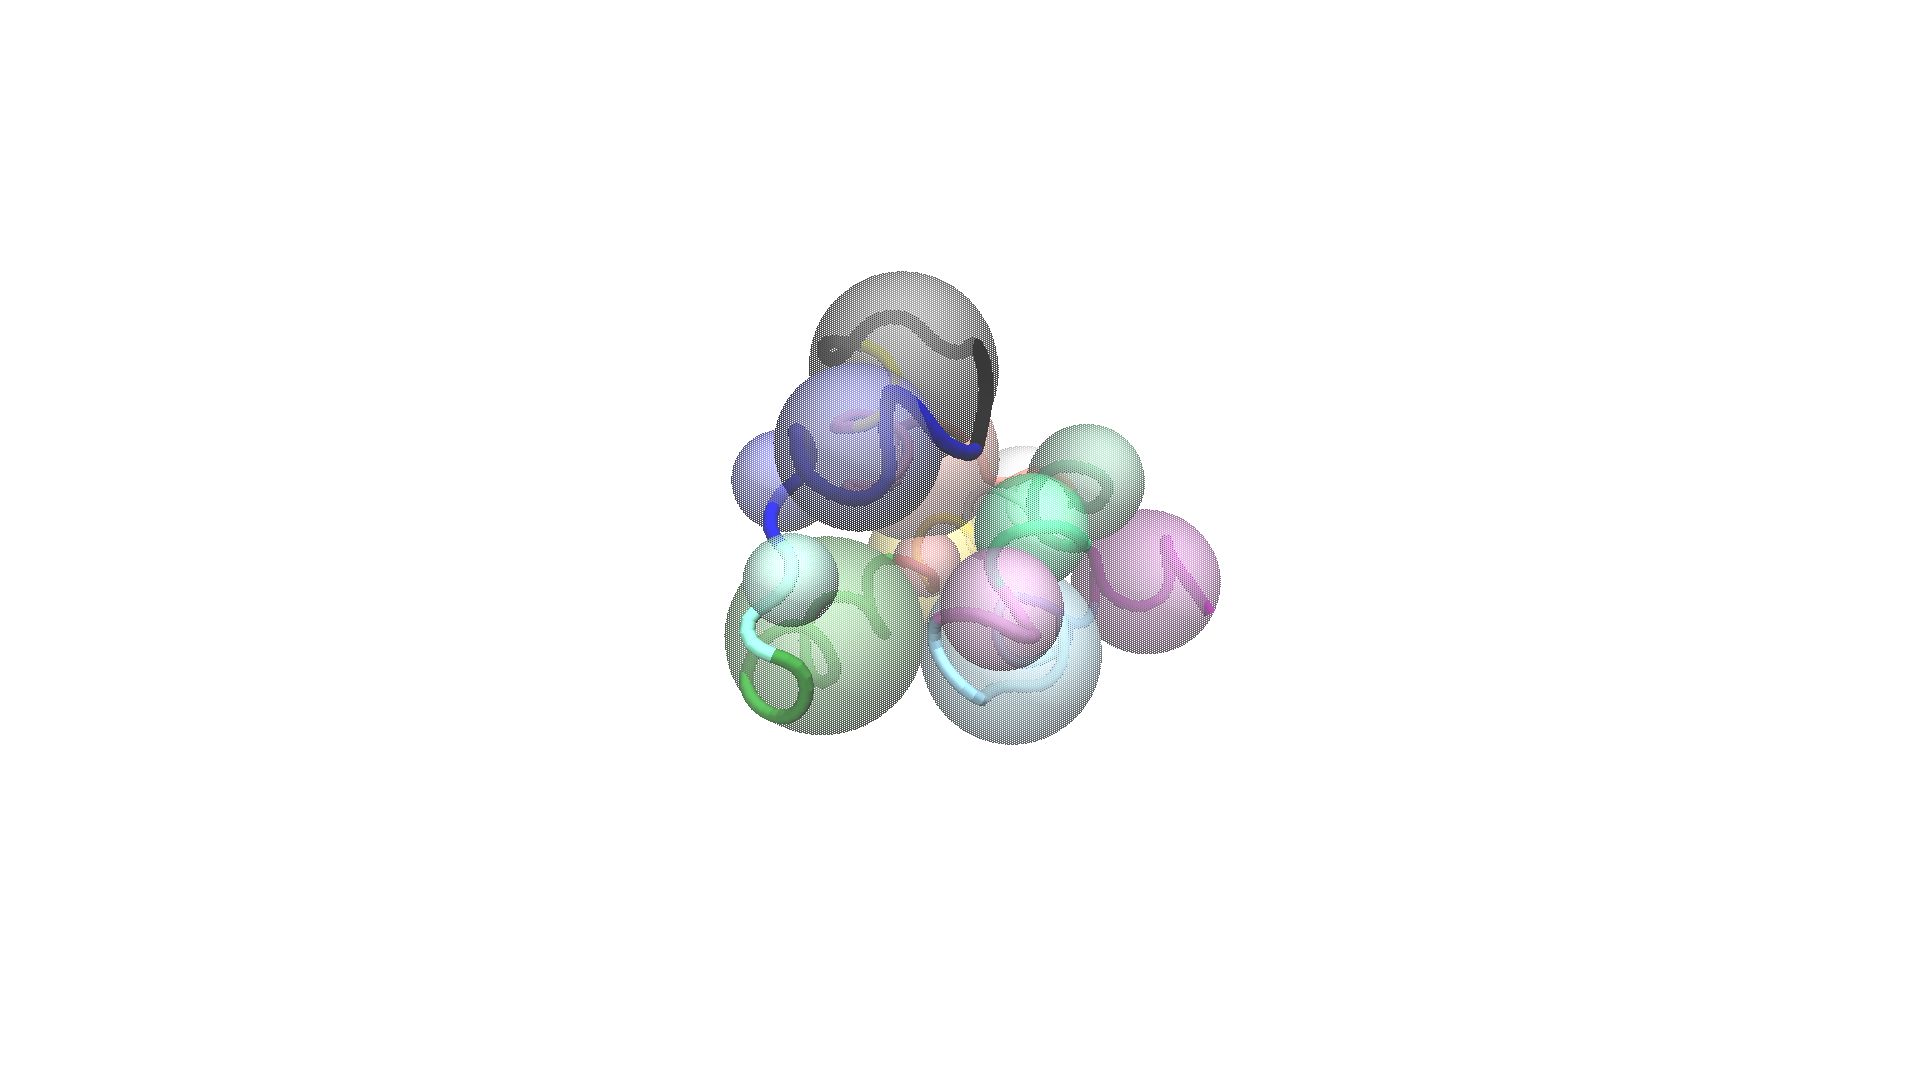
\includegraphics[width=0.25\textwidth, trim={22cm 6cm 22cm 6cm},clip]{lambda_repressor_beads.png}}
  \caption{\label{all_beads}Decomposition results of the 10 fast-folding proteins in the order of protein's size. The structures shown here are representatives selected from the folded metastable states we identified from the simulation data. And the different colors indicate the different assembly units. The transparent spheres over there are to give a concept that these units can be the candidates of a CG model. They are plotted with the center of masses of all heavy atoms within the unit and the radius of gyration of them.}
\end{figure}

{\bf Larger Molecule, Larger Assembly Units.} To check the consistency of the results from different proteins, we first calculate the average size (in a measurement of heavy atom number) of the minimal assembly units for each protein as a general statistics. Then we plot the average size against the total heavy atom number of the corresponding protein. Here, we also plot the data points of FIP35 and NTL9, the two proteins tested in the original paper of S3D\cite{Lrenzo_S3D}, so in fig-\ref{all_stat}, there are 12 data points in total. We find there is a trend that roughly larger proteins will also have larger assembly units. This is reasonable because as the molecule becomes larger, specific local fluctuations will have less influence on the global conformational movements. As a result, for most proteins investigated here, their average size of assembly units is between 20 to 30 heavy atoms. However, there are two proteins whose results are outside of the normal range: homeodomain's assembly units seem to be much larger than other proteins and $\alpha 3D$'s much smaller. This is because the dynamics of these two proteins are different from others, which we will discuss below.

\begin{figure}[htbp]
  \centering
  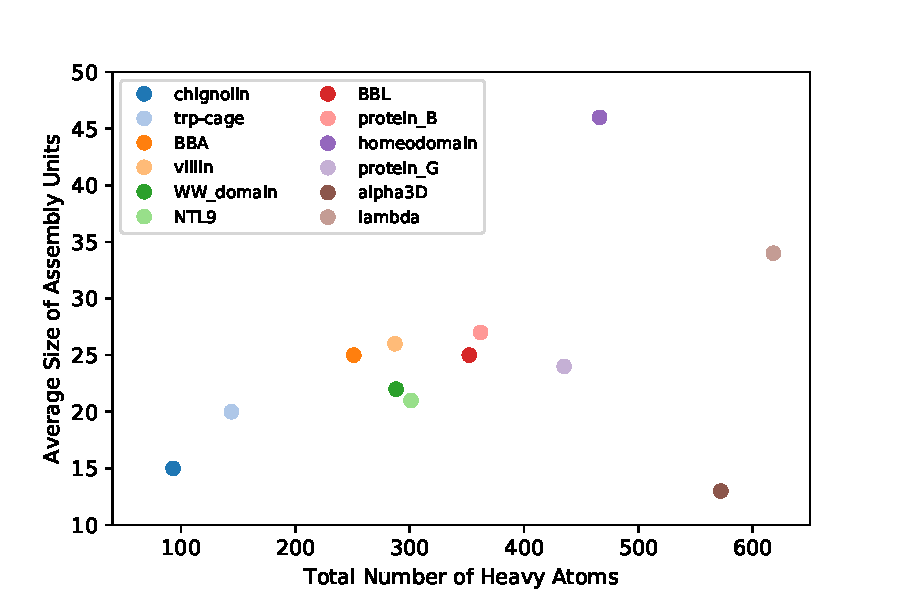
\includegraphics[width=1\textwidth]{stat_size_color.pdf}
  \caption{\label{all_stat}Average sizes of the assembly units against the sizes of all the proteins}
\end{figure}

{\bf Homeodomain Doesn't Unfold Completely.} The simulation data of homeodomain we use is actually not from a natural protein, but a designed mutant called UVF\cite{DE_Shaw_fast-folding}. The stability of UVF has been strengthened so much that its unfolding transition will not complete even under 99$^{\circ}$C\cite{UVF_earlier,UVF_origin}. In our calculation, we identified 3 metastable states for homeodomain, which correspond to the unfolded, intermediate and folded state. In fig-\ref{UVF}, we show the contact probability of these 3 metastable states, which clearly indicates that in all states homeodomain's 3 cores of $\alpha$-helices are formed, {\it i.e.} the folding process mainly takes place on the tertiary structure. The stability of its secondary structure causes 2 results: 1) the conformation is always very compact, which leads to a small number of coherent domains for each metastable state; 2) the relatively high structural similarity of these 3 states' makes their coherent domains very similar, {\it i.e.} there are more common boundary positions of coherent domains from different states, so the splittings and mergings become less during the interstate transition. As a consequence of these 2 factors, it is reasonable that we obtained less and larger minimal assembly units from this protein.

\begin{figure}[htbp]
  \centering
  \subfloat[Unfolded State]{
  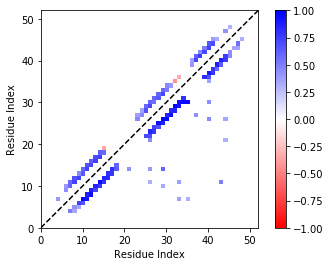
\includegraphics[width=0.33\textwidth]{UVF_contact_HMM_3_state_2_10TICA.png}}
  \subfloat[Intermediate State]{
  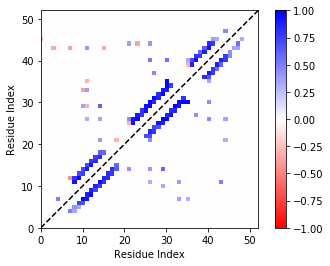
\includegraphics[width=0.33\textwidth]{UVF_contact_HMM_3_state_0_10TICA.png}}
  \subfloat[Folded State]{
  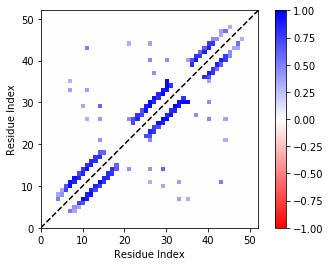
\includegraphics[width=0.33\textwidth]{UVF_contact_HMM_3_state_1_10TICA.png}}
  \caption{\label{UVF}Contact probability of the 3 metastable states of homeodomain (above diagonal) against the folded state (below diagonal). Blue indicates native contacts and red the non-native ones. Cutoff distance for contact formation is 0.4 nm. Only contacts formed in over $30\%$ frames are shown.}
\end{figure}

{\bf The Dynamics of $\alpha 3D$ is Frustrated.} $\alpha 3D$ is a {\it de novo} designed protein\cite{A3D_de_novo}. Though its folding process is very fast\cite{A3D_fast_folder}, the dynamics is relatively frustrated. Best, {\it et al.} have demonstrated that $\alpha 3D$'s native contacts are not remarkably preferred during the folding process by using 1) a log-ratio of lifetimes of contacts on transition paths (TP) and unfolded state; and 2) a Bayesian measure of how predictive the formation of each contact is for being on a TP. Specifically, it was demonstrated that not like other natural proteins, nonnative contacts also play an important role in the folding mechanism determination of $\alpha 3D$\cite{A3D_frustration}. In our calculation, we identified 5 metastable states for $\alpha 3D$, which is the highest number among the test set. we also found that there are 2 metastable states that are well-folded with a difference in the second loop region as shown in fig-\ref{A3D_contact}. From the calculation of frustratometer, these contacts are all highly frustrated\cite{Justin_frustration}. In addition, we haven't observed similar multiple folded state phenomenon on other proteins. Both of these results show that the dynamics of $\alpha 3D$ is more frustrated than other good folders, therefore, different regions of the molecule are less dynamically correlated. As a result, we need more and smaller assembly units (a finer mapping) to capture its long-timescale dynamics. 

\begin{figure}[htbp]
  \centering
  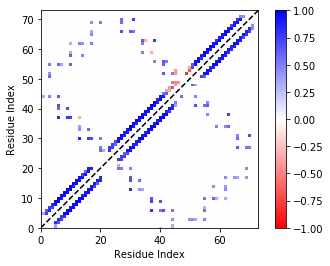
\includegraphics[width=0.5\textwidth]{A3D_contact_HMM_5_state_4_contacts.png}
  \caption{\label{A3D_contact}The contact maps of the 2 folded metastable states of $\alpha 3D$. Since the state shown in the below diagonal has the same structure in the second loop as the structure measured (PDB ID: 2A3D), we chose it as the native state. Blue indicates native contacts and red the non-native ones. Cutoff distance for contact formation is 0.4 nm. Only contacts formed in over $30\%$ frames are shown.}
\end{figure}

\subsection{Intrinsically Disordered Proteins}

{\bf A Modified Version of S3D for IDPs.} Besides fast-folding proteins, we also perform decomposition for 2 intrinsically disordered proteins. We found that S3D could not be directly applied on IDPs. Modification is needed to extend applications on IDPs. The issue is caused by the dynamics of IDPs, which is different from folded proteins. Since IDPs are very flexible and don't have specific folded structures\cite{IDP,IDP_TOMPA}, we cannot identify the metastable states as we did before\cite{IDP_dynamics}. However, because IDPs' dynamical characteristics will change under different conditions (such as different denaturant concentrations), we think that it makes sense to use time-averaged diffusion map\cite{Lrenzo_S3D} to perform decomposition on the simulation data under different conditions, then combine these results to obtain the minimal assembly units as their intersection. To accomplish this, we replace the metastable states with trajectories from different simulations.

We illustrate this modified S3D on 2 IDPs, ACTR and MYC. The simulation data we use contains 6 $2\mu s$-long trajectories of ACTR under different urea concentrations\cite{ACTR} and 4 trajectories of MYC with length varies between $2-3\mu s$ under different NaCl concentrations\cite{MYC}. The minimal assembly units of these 2 IDPs are shown in fig-\ref{IDP_all_beads}. The coherent domains of each trajectory can be found in the supplementary material. The number of assembly units is again much less than the number of residues, which indicates the long-timescale dynamics of proteins mainly happens on a spacial scale that is above single residue. The results from these 2 IDPs are consistent with each other as well. The average sizes of their assembly units are quite similar.

\begin{figure}[htbp]
  \centering
  \subfloat[ACTR]{
  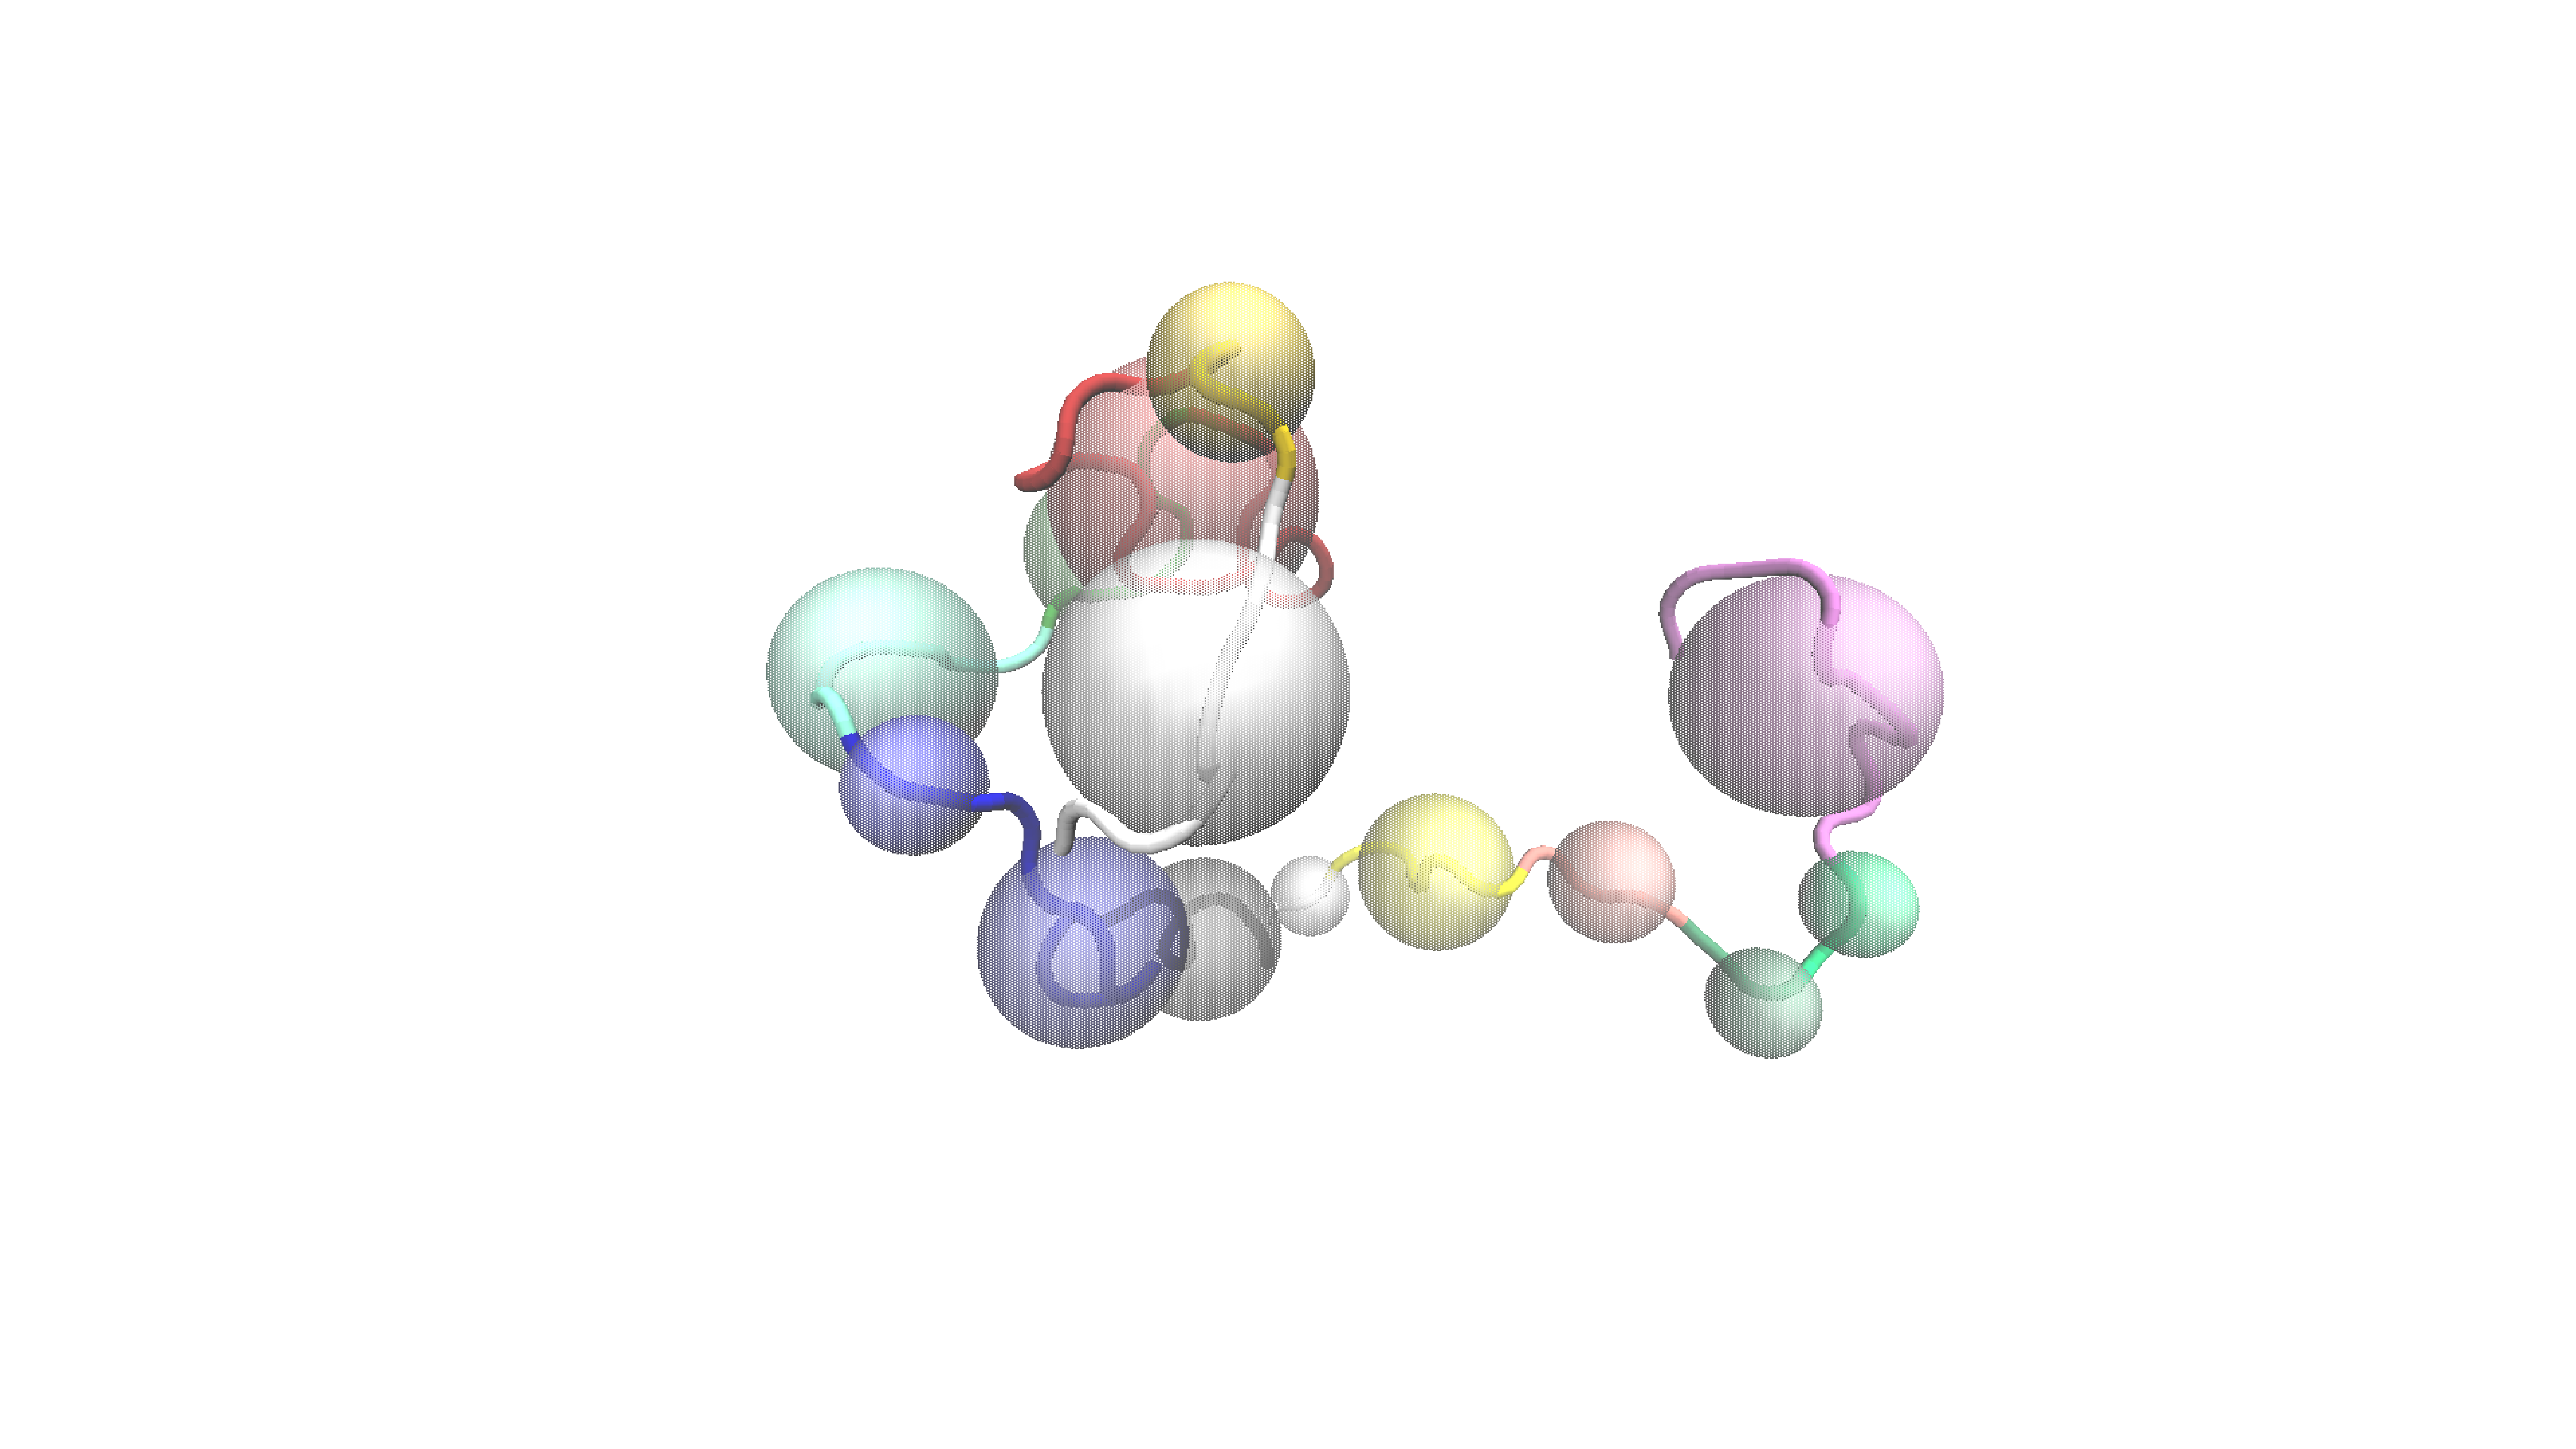
\includegraphics[width=0.5\textwidth, trim={35cm 18cm 35cm 18cm},clip]{ACTR_all_beads.png}}
  \subfloat[MYC]{
  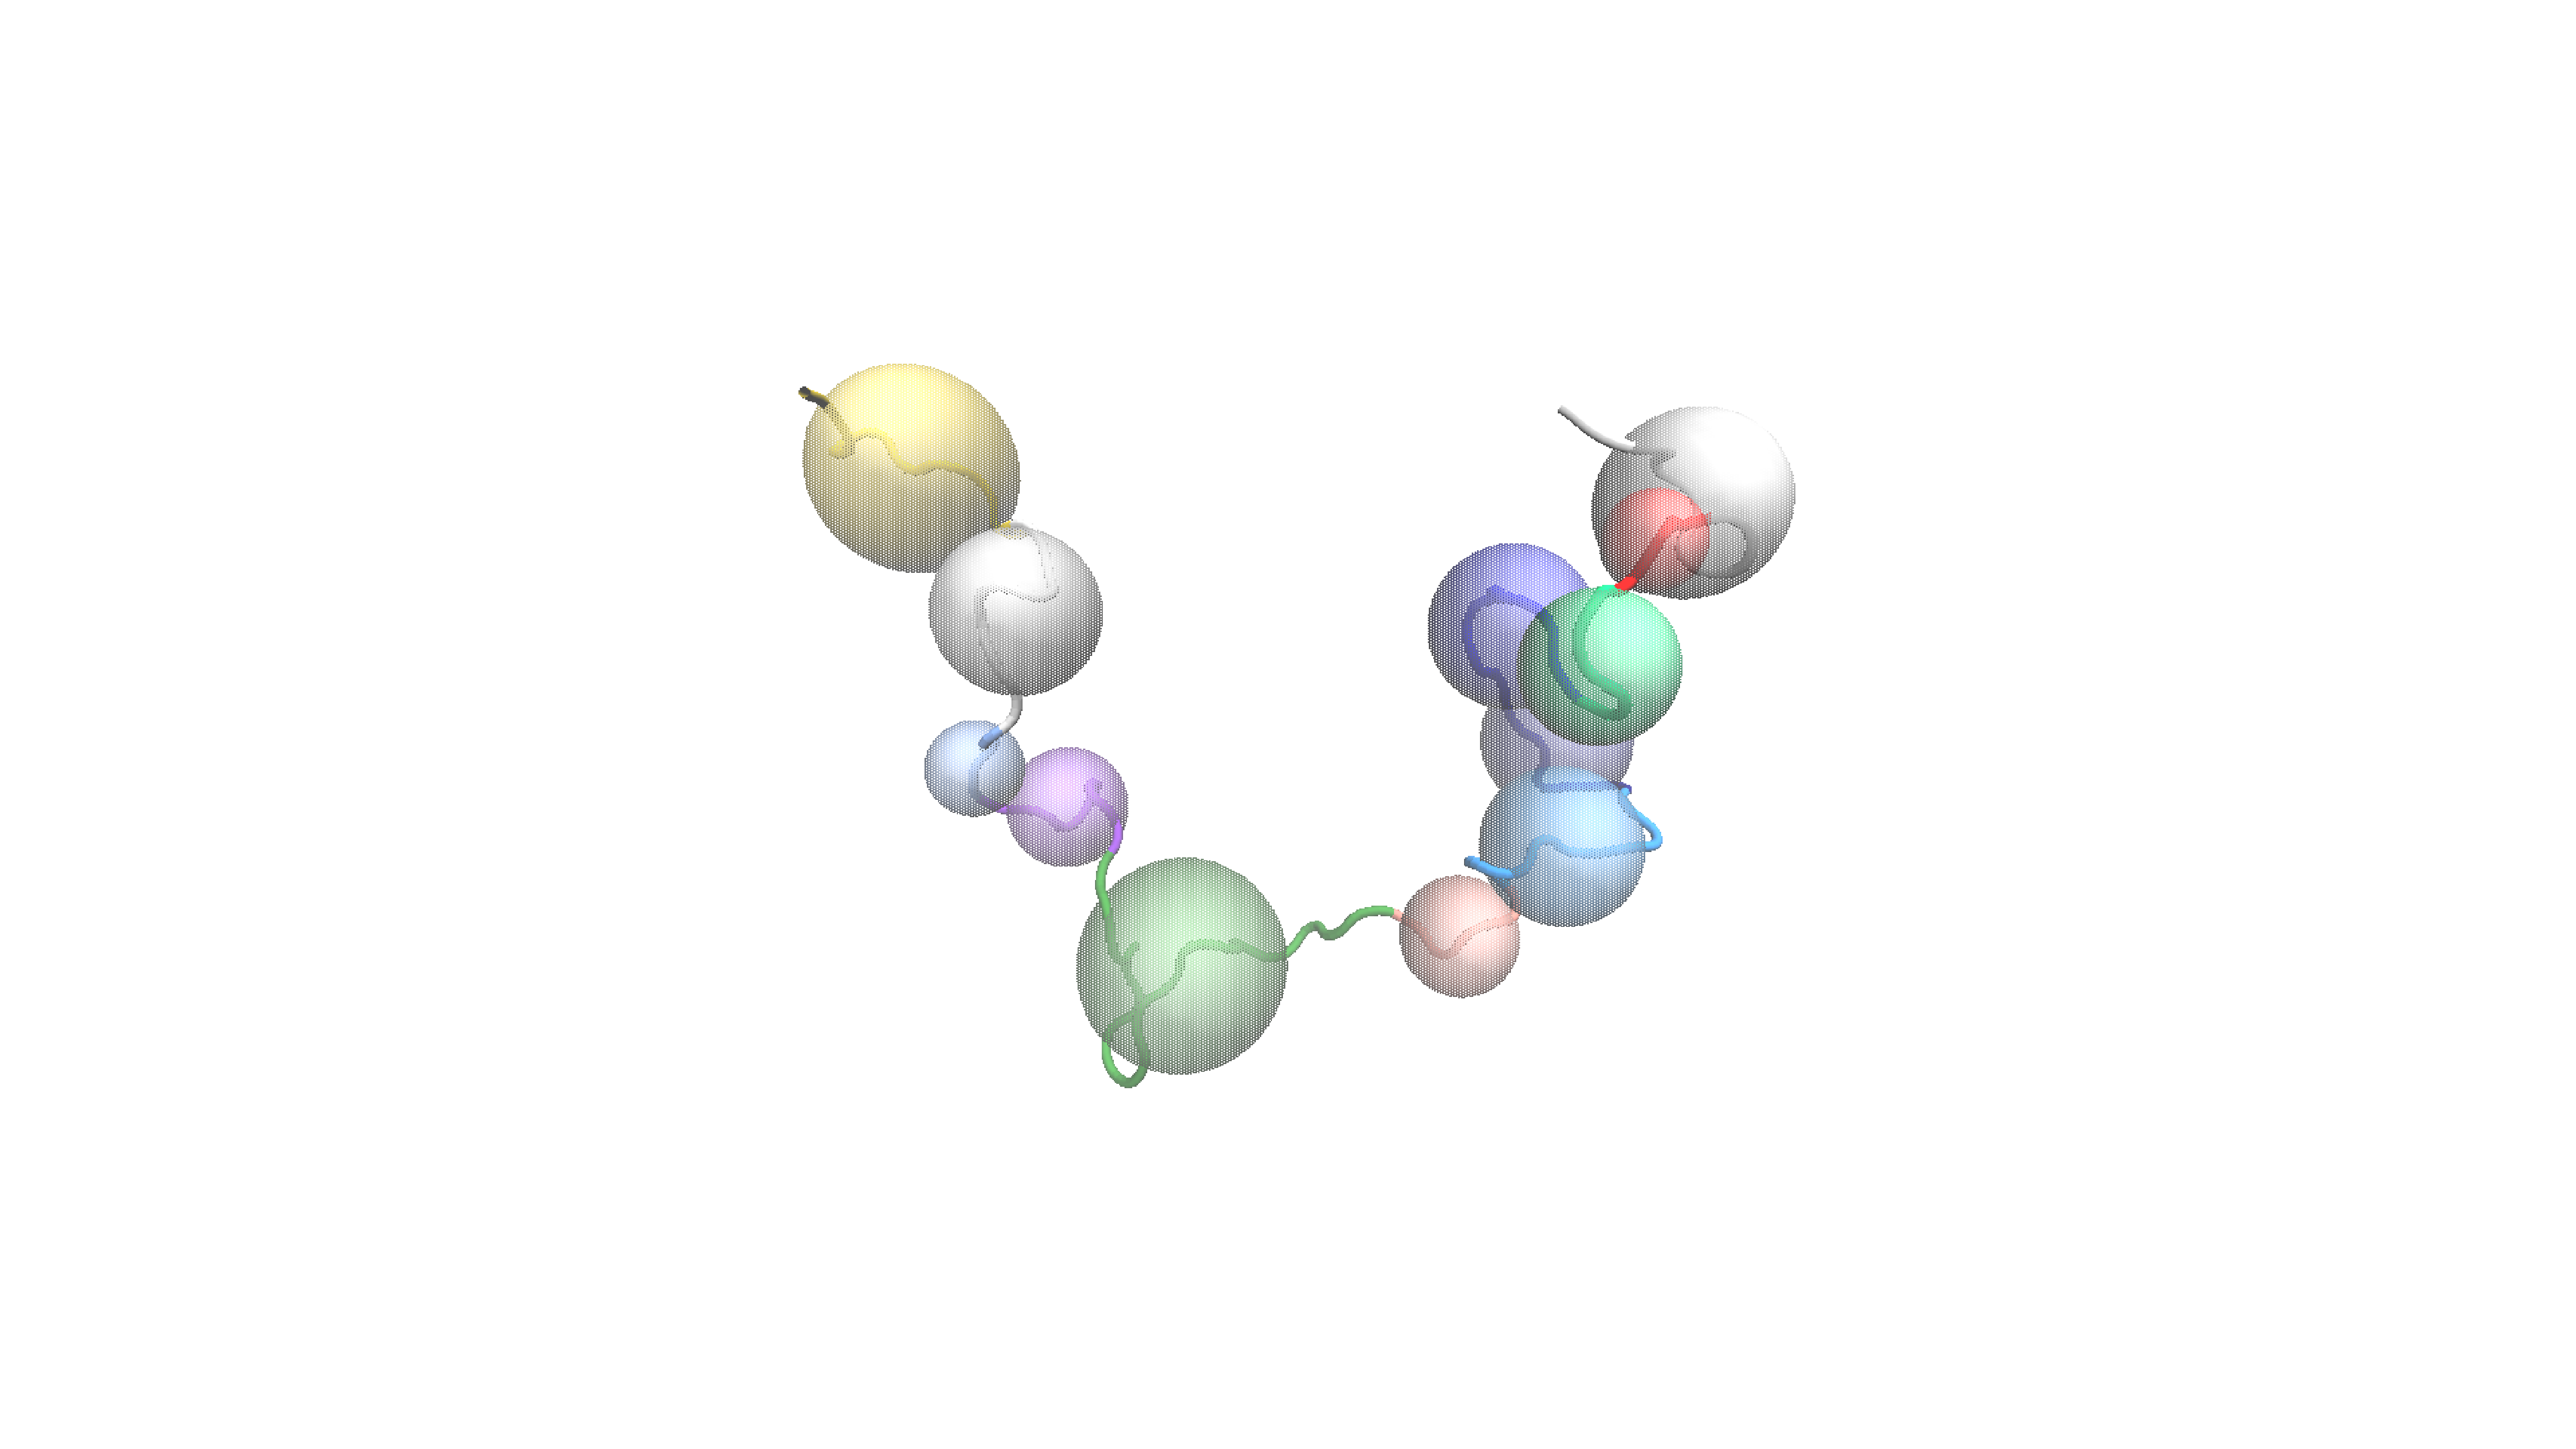
\includegraphics[width=0.5\textwidth, trim={35cm 18cm 35cm 18cm},clip]{MYC_all_beads.png}}
  \caption{\label{IDP_all_beads}The minimal assembly units of the 2 IDPs. The structures shown here are representatives selected from the trajectories with the lowest concentration of solute (0M urea for ACTR, 0.1M NaCl for MYC).}
\end{figure}

{\bf Convergence of the Assembly Units Number.} However, not like folded proteins who have a limited number of metastable states, the number of different simulations for IDPs can be very large. Thus, whether the increasing amount of data will lead to more and more assembly units or there will be an upper bound becomes a question worths investigation. To answer this question, we use different amounts of the simulation data, and see how will the number of assembly units change as the amount of used data increases. In practical, with the coherent domains under all the conditions obtained, we calculate the average number of assembly units needed for all the possible combination of a sub-dataset with N simulations. The curves of average assembly units number against the size of the sub-dataset, N, is shown in fig-\ref{IDP_N_units}. While we didn't observe an obvious convergence of the assembly units number as the amount of used data increases. This may be caused by one of these two factors: 1) probably it's because the data we have is not enough, since there's a trend that the growth of assembly units number is slowing down as we use more simulations; 2) also, there might be no upper bound of the assembly units number for IDPs, because they have very different behaviors under different conditions. Whichever of these is true, it is sure that it's difficult to obtain a set of minimal assembly units works universally for IDPs, because it is either impossible or needs a large amount of data. 

\begin{figure}[htbp]
  \centering
  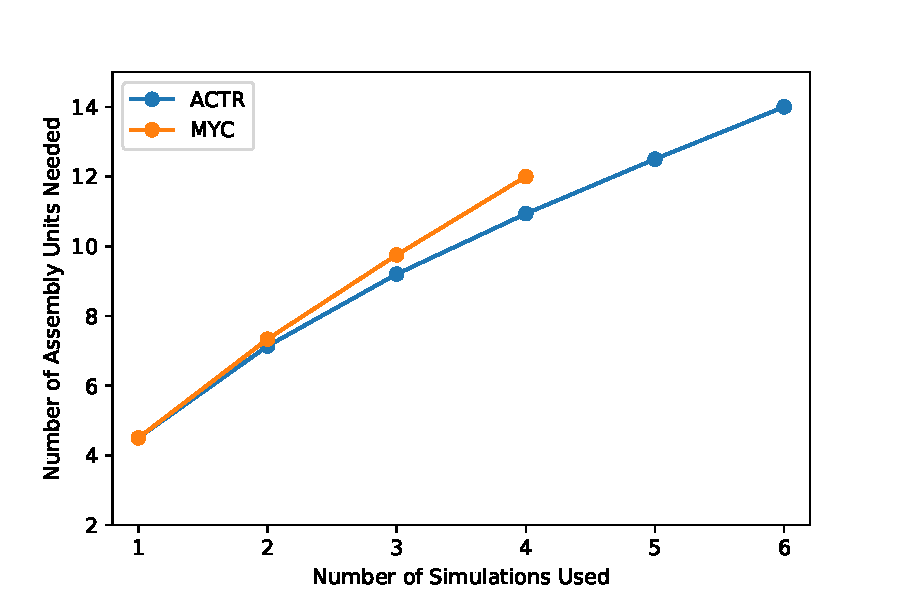
\includegraphics[width=1\textwidth]{IDP_N_units.pdf}
  \caption{\label{IDP_N_units}The average number of assembly units needed against the number of simulations used as dataset.}
\end{figure}

\section{Conclusion}

By applying the {\it Structure and State Space Decomposition} algorithm\cite{Lrenzo_S3D} on a set of 10 fast-folding proteins and 2 intrinsically disordered proteins, we demonstrate that the dynamics of proteins has a crucial influence on the coherency of different parts of its molecule. For common fast-folding proteins with a size around 50 residues, their assembly units will have an average size locates between 20 to 30 heavy atoms. As the protein becomes larger, local fluctuations will have less influence on the global conformational change, which leads to larger assembly units. While if the dynamics is abnormal in someway, the decomposition result will also change correspondingly. The conformational change of homeodomain is relatively small, thus it has larger and less assembly units. However, because the dynamics of $\alpha 3D$ is highly frustrated, different parts of the molecule are less dynamically correlated.

Moreover, we also propose a modified version of S3D for IDPs, because their different dynamics makes Markov state model analysis inapplicable. Thus, we use the simulation data under different conditions as an analogue of the metastable states of folded proteins to complete the decomposition. However, because IDPs' behavior will change with the condition, we found as the amount of input simulation data grows, more and more assembly units will be needed. We didn't observe an obvious convergence in this process. Thus, we conclude that it's difficult to find a set of minimal assembly units that works universally for IDPS, {\it i.e.} the dynamical coherency between different parts of IDP molecules is weak.

Finally, as an outlook of this algorithm, since the minimal assembly units obtained with S3D is a good candidate of effective atoms for coarse-grained models, it is possible to develop a corresponding force filed to construct a totally data-driven CG model at least for folded proteins. We believe such a model will provide us a new perspective of view on coarse-grained modeling. For intrinsically disordered proteins, we may also construct such models by restricting the condition to control the number of assembly units. Furthermore, the decomposition result itself may also provide us inspirations on the relation between protein's structure and functions.

%%%%%%%%%%%%%%%%%%%%%%%%%%%%%%%%%%%%%%%%%%%%%%%%%%%%%%%%%%%%%%%%%%%%%
%% The "Acknowledgement" section can be given in all manuscript
%% classes.  This should be given within the "acknowledgement"
%% environment, which will make the correct section or running title.
%%%%%%%%%%%%%%%%%%%%%%%%%%%%%%%%%%%%%%%%%%%%%%%%%%%%%%%%%%%%%%%%%%%%%
\begin{acknowledgement}

We are grateful to D. E. Shaw Research for sharing the simulation data used in the work.  Wangfei want to thank all the members of Dr. Clementi's group for their assistance, especially for the introduction of S3D algorithm from Lorenzo Boninsegna, and the helpful discussions on Markov state model analysis with Feliks Nüske. 

\end{acknowledgement}

%%%%%%%%%%%%%%%%%%%%%%%%%%%%%%%%%%%%%%%%%%%%%%%%%%%%%%%%%%%%%%%%%%%%%
%% The same is true for Supporting Information, which should use the
%% suppinfo environment.
%%%%%%%%%%%%%%%%%%%%%%%%%%%%%%%%%%%%%%%%%%%%%%%%%%%%%%%%%%%%%%%%%%%%%
\begin{suppinfo}

The Supporting Information is available. Details about the S3D work flow, metastable states and the corresponding clustering results.

\end{suppinfo}

%%%%%%%%%%%%%%%%%%%%%%%%%%%%%%%%%%%%%%%%%%%%%%%%%%%%%%%%%%%%%%%%%%%%%
%% The appropriate \bibliography command should be placed here.
%% Notice that the class file automatically sets \bibliographystyle
%% and also names the section correctly.
%%%%%%%%%%%%%%%%%%%%%%%%%%%%%%%%%%%%%%%%%%%%%%%%%%%%%%%%%%%%%%%%%%%%%
\bibliography{bib}

\end{document}
